% !TEX root = thesis.tex



\chapter{Measuring Dynamic Dense 3D Surface Movements}
\label{chapter:trajectory}

Important messages during communication are often transmitted by subtle body movements. Accurately measuring such body movements in 3D across time is therefore important in analyzing social interactions. In this chapter, we aim at reconstructing dense 3D trajectories of dynamic 3D object, which we refer to as a \emph{3D trajectory stream}. However, such video-based 3D motion reconstruction is challenging, as natural motion produces a greater occurrence of measurement loss due to occlusion and also causes artifacts in imagery (e.g., motion blur and texture deformation). Utilizing a large number of cameras can address these challenges, because it is likely to (1) narrow the average baseline between nearby cameras, (2) reduce the occurrence of occlusion, and (3) provide robustness to measurement noise due to the surplus views. However, previous approaches are unable to fully leverage the increasing number of views to improve 3D tracking performance (in terms of the average length of reconstructed trajectories, the density of the trajectories, and the accuracy of localization). The principal cause of failure emerges from errors in reasoning about the time-varying \emph{visibility} of dynamic 3D points. Poor visibility reasoning severely affects tracking performance, as an algorithm cannot benefit from an alternate viewpoint if it is unaware that the point is visible in the alternate view. Furthermore, an erroneous conclusion that a point is visible in a camera can bias the reconstruction, often producing a characteristic ``jump" artifact where a point assumes the identity of a different location.


%Thousands of images exist for most significant landmarks around the world. The availability of such imagery has facilitated the development of large-scale 3D reconstruction algorithms, which fully leverage the number of views to produce dense and accurate 3D point clouds~\cite{Snavely:2006,Frahm:2010,Furukawa:2010}. Increasingly, landmark \emph{events} are also being captured at scale by hundreds of cameras at major sports games, concerts, and political rallies. However, analogous large-scale reconstruction algorithms, that are able to fully leverage a large number of views of an event to produce long, dense, and accurate 3D trajectories, do not yet exist. %In this paper, we present a method for reasoning about the visibility of the target points at each camera view, to reconstruct the 3D motion of a dynamic scene from a large number of views.



%Existing approaches have addressed these challenges through structural regularization, either by assuming a fixed topology \cite{Furukawa2008, Beeler2011} or by spatially regularizing the trajectories \cite{Basha2012a,Huguet2007,Vogel2011}. However, the performance of such approaches are usually limited in terms of accuracy and density of the reconstructed motion trajectories, due to the and they are failed in producing practically applicable 3D motion due to the limitation of measurement and over-regularization available information. 
%have been proposed usually in a limited system setup with relatively small number of cameras, as shown in Table~\ref{Table:camSettup}. 

%Following static reconstruction algorithms, existing approaches reason about visibility (if at all) assuming photometric consistency among cameras where the target point is visible \cite{Carceroni2002,Devernay2006,Furukawa2008}: if the local appearance of a point matches the expected appearance, it is considered visible in that camera. However, photometric consistency tends to require frontal facing cameras (with respect to the tangent plane at the point), are susceptible to imaging artifacts, and require accurate estimates of the tangent plane normal at the point. Poor visibility reasoning severely affects tracking performance and obstructs the full benefit of a large number of unique viewpoints. 

In this chapter, we demonstrate a method that precise inference of point visibility allows reconstruction algorithms to fully leverage large numbers of views to produce longer 3D trajectories with higher accuracy. In particular, our core algorithmic contributions in this chapter are: (1) the use of motion consistency as a cue for the visibility of moving points; (2) the use of viewpoint regularity as a prior and a measure for viewpoint proximity; and (3) a maximum a posteriori (MAP) estimate for visibility estimation by probabilistically incorporating these cues with photometric and geometric consistency. We report empirical performance in reconstructing 3D motion captured by 480 VGA cameras\footnote{This research was conducted before we build the HD and RGB+D sensors in the Panoptic Studio} in scenes that contains significant occlusion, large displacement, and changes in the topology of the scene.

\begin{figure}[t]
	\begin{center}
		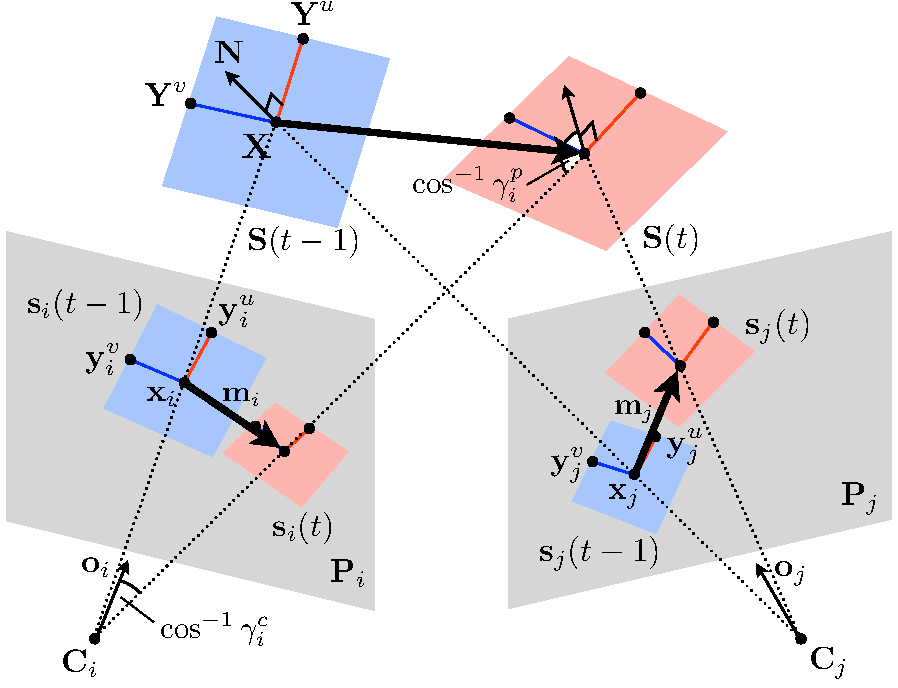
\includegraphics[width=0.6\linewidth]{figures/Notation_final}
		\caption{The motion of a patch between time $t-1$ and $t$ is reconstructed from multiple cameras.}
		\label{fig:notation}
	\end{center}
\end{figure}
%\interfootnotelinepenalty=10000
%\vspace{-0.2cm}
\section{Notation}
%\vspace{-0.2cm}
Our algorithm takes, as input, image sequences from $N$ calibrated and synchronized cameras over $F$ frames and produces, as output, 3D trajectories of $P$ moving points with their instantaneous orientations and associated visibility in each camera frame. Since the method is applied to each point independently, we consider only a single point here to simplify the exposition.

As shown in Figure~\ref{fig:notation}, we track a parallelogram patch centered on a target 3D point $\mathbf{X} \in \mathds{R}^3$, whose extent is defined by two additional points $\mathbf{Y}^u$ and $\mathbf{Y}^v \in \mathds{R}^3$. The texture information $\mathbf{Q} \in \mathds{R}^m$ associated with the patch is defined by a unit vector concatenating normalized intensity values at a fixed number of grid positions on the patch, where $m$ is the number positions in the grid\footnote{The texture vector $\mathbf{\mathbf{Q}}$ is normalized as follows:
	\begin{eqnarray}
	\mathbf{Q} = \frac{1}{\sqrt{\sum_{j=1}^m (Q_j-\overline{Q})^2}} \left[\begin{array}{c}Q_1-\overline{Q}\\\vdots\\ Q_m-\overline{Q} \end{array}\right] \label{Eq:normalized_texture}
	\end{eqnarray}
	where $\overline{Q} = \sum_{j=1}^m Q_j / m$ and $Q_j$ is the $j^{\textrm th}$ intensity value of the texture.}. 

The patch $\mathbf{S}(t)$ is denoted by the set $\{\mathbf{X}(t), \mathbf{Y}^u(t), \mathbf{Y}^v(t),\mathbf{Q}(t)\}$, which is associated with the camera visibility set $\mathbf{V}(t) = \{\mathbf{v}_1(t),\cdots,\mathbf{v}_N(t)\}$, where $\mathbf{v}_i(t)$ is a binary value representing visibility with respect to  the $i^{\textrm th}$ camera. % The normal $\mathbf{N}(t)$ is a unit vector orthogonal to the patch.
%\begin{equation}
%\mathbf{N}(t)= \frac{\left(\mathbf{Y}^u(t) - \mathbf{X}(t)\right) \times \left(\mathbf{Y}^v(t) - \mathbf{X}(t)\right)} {\left\| \left(\mathbf{Y}^u(t) - \mathbf{X}(t)\right) \times \left(\mathbf{Y}^v(t) - \mathbf{X}(t)\right) \right\|}. \nonumber
%\end{equation}
A 3D point is projected onto the $i^{\textrm th}$ camera associated with a $3\times4$ projection matrix $\mathbf{P}_i$. The projection matrix is parametrized by a camera center vector $\mathbf{C}_i \in \mathds{R}^3$ and a 3$\times$3 rotation matrix $\mathbf{R}_i \in SO(3)$. The ``look-at" vector $\mathbf{o}_i$ is aligned with the $z$-axis of the camera, i.e., the third column of $\mathbf{R}_i^\mathsf{T}$. 

The 3D patch is projected onto the camera plane to form the projected patch $\mathbf{s}_i(t) = \{\mathbf{x}_i(t), \mathbf{y}_i^u(t), \mathbf{y}_i^v(t), \mathbf{q}_i(t) \}$, where $\mathbf{x}_i(t)$, $\mathbf{y}^u(t)$, and $\mathbf{y}^v(t) \in \mathds{R}^2$ are the projected points, i.e., $\widehat{\mathbf{x}}_i(t) \cong \mathbf{P}_i \widehat{\mathbf{X}}(t)$, $\widehat{\mathbf{y}}_i^u(t) \cong \mathbf{P}_i \widehat{\mathbf{Y}}^u(t)$, and $\widehat{\mathbf{y}}_i^v(t) \cong \mathbf{P}_i \widehat{\mathbf{Y}}^v(t)$, where $\widehat{\cdot}$ is the homogeneous coordinate representation of each vector. $\mathbf{q}_i  \in \mathds{R}^m$ is the texture information of the projected patch, which is defined by a concatenation of all the intensities from the $i^{\textrm th}$camera, corresponding to the projected grid positions of $\mathbf{S}$, and normalized as in Equation~(\ref{Eq:normalized_texture}). Ideally, $\mathbf{Q}=\mathbf{q}_i$ if the 3D patch $\mathbf{S}$ is visible from the $i^{\textrm th}$ camera, discounting illumination variation. We denote $\mathbf{m}_i$ as 2D optical flow at $\mathbf{x}_i(t-1)$ in the $i^{\textrm th}$ camera, as shown in Figure~\ref{fig:notation}. 

The relationship between the $i^{\textrm th}$ camera and patch can be defined by the co-visibility set $\mathbf{\Gamma}_i = \{\gamma^c_i, \gamma^p_i\}$, where
\begin{eqnarray}
\gamma^c_i = \frac{ (\mathbf{X}-\mathbf{C}_i)^\mathsf{T}\mathbf{o}_i} { || \mathbf{X}-\mathbf{C}_i || }~~~{\textrm and}~~~\gamma^p_i = \frac{ (\mathbf{C}_i - \mathbf{X})^\mathsf{T}\mathbf{N}} { || \mathbf{C}_i - \mathbf{X} || }, \nonumber
\end{eqnarray}
$\gamma^c_i$ encodes the angle cosine of the patch location with respect to the camera ``look-at" vector $\mathbf{o}_i$ and $\gamma^p_i$ encodes the angle cosine of the camera location with respect to the 3D patch normal $\mathbf{N}$.

% In the tracking process, we compute 2D optical flow $\mathbf{m}_i$ at $\mathbf{x}_i(t-1)$ in the $i^{\rm th}$ camera as shown in Figure~\ref{fig:notation}. 


% We also define a scalar value $\gamma_i$ for the $i^{\rm th}$ camera representing the relationship between the camera center position and patch normal direction, as
% \begin{equation}
% \gamma_i = \frac{ (\mathbf{C}_i - \mathbf{X})^\mathsf{T}\mathbf{N}} { || \mathbf{C}_i - \mathbf{X} || }.
% \end{equation}
% A negative valued $\gamma_i$ means that the $i^{\rm th}$ camera center is located behind the patch.

\begin{figure}[t]
	\centering
	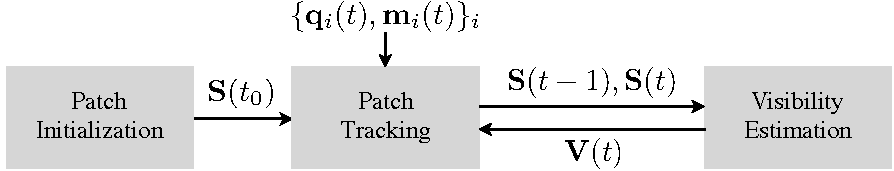
\includegraphics[width=0.7\linewidth]{figures/FlowChart}
	\caption{Overview of patch tracking and visibility estimation.}
	\label{fig:overview}
\end{figure}

%\vspace{-0.2cm}
\section{Overview}
%\vspace{-0.2cm}
At the initial time instance $t_0$, a target 3D patch is reconstructed and, over time, the algorithm alternately estimates the patch position and normal and its visibility with respect to all cameras. It should be noted that $t_0$ can be any arbitrary frame and that the tracking and the visibility computation are performed both forwards and backwards in time from $t_0$. We consider only forward tracking, from $t-1$ to $t$ to simplify the description. The flow chart of our algorithm is shown in Figure~\ref{fig:overview}.

\noindent \textbf{Patch Initialization.} Given the images from different cameras at the same time instance $t_0$, the algorithm reconstructs 3D points by matching features and triangulates them within a RANSAC framework. A 3D patch centered on $\mathbf{X}$ is reconstructed by maximizing the photometric consistency among the cameras where the patch is visible\footnote{The cameras that participate in RANSAC are used as an initial visible set, and the reference camera $\mathbf{P}_{\textrm{ref}}$ is selected as the one closest to the initial 3D point in the iniler set. A 3D patch centered on $\mathbf{X}$ is initialized as a fixed scale square patch (40mm$\times$40mm), with $\mathbf{N}$ parallel to $\mathbf{o}_{\textrm ref}$. We refine the patch based on the method described by Furukawa and Ponce~\cite{Furukawa2010} and select a new reference camera as the one closest to the current patch normal. The corresponding visibility set is updated by selecting cameras that have higher Normalized Cross Correlation (NCC) score than a threshold compared to $\mathbf{P}_{\textrm{ref}}$. Within the patch initialization process, the normal refinement and visibility update are iterated.}. This initializes $\mathbf{S}(t_0)$ and $\mathbf{V}(t_0)$.

\noindent \textbf{Patch Tracking.} Given the previously obtained 3D patch $\mathbf{S}(t-1)$ and visibility $\mathbf{V}(t-1)$, the algorithm estimates the next 3D patch $\mathbf{S}(t)$ based on 2D optical flow in the cameras defined by $\mathbf{V}(t-1)$. For the $i^{\textrm th}$ camera in $\mathbf{V}(t-1)$, optical flow~\cite{Lucas1981} is estimated at multiple scales at the points $\mathbf{x}_i(t-1)$, $\mathbf{y}^u_i(t-1)$, and $\mathbf{y}^v_i(t-1)$. To eliminate unreliable flow, a backward-forward consistency check~\cite{sundaram2010dense} is performed for flow at each scale and only the most reliable flow is retained. The next 3D positions, $\mathbf{X}(t)$, $\mathbf{Y}^{u}(t)$, and $\mathbf{Y}^{v}(t)$, are estimated by triangulating optical flow outputs within a RANSAC framework. The RANSAC process is crucial since $\mathbf{V}(t-1)$ may not be valid anymore at time $t$, due to motion. After RANSAC, the normal is refined by maximizing the photometric consistency among the images that belong to the inliers of RANSAC, as in the patch initialization process.

% ignored footnote
%\footnote{In practice, optical flow is computed from all the images regardless membership of visibility, since, in the end, it is used to compute the visibility likelihood based on motion-based consistency for all the cameras, as described in \ref{sub:Motion-Cue}}

\noindent \textbf{Visibility Estimation.} Based on the reconstructed $\mathbf{S}(t)$ and its motion from $\mathbf{S}(t-1)$, our approach finds the MAP estimate of the current visibility set $\mathbf{V}(t)$ by fusing photometric consistency, motion consistency, and geometric consistency, in conjunction with a Markov Random Field (MRF) prior. Typically, the tracking process is severely affected by false positive cameras where the target is not visible. Poor visibility reasoning at the RANSAC stage can cause a characteristic ``jump" error to a different scene point, and also reduces the normal refinement performance causing frequent local minima during the optimization process. Our precise visibility estimation results in longer trajectories of higher accuracy.

Patch tracking and visibility estimation are interdependent processes. At each time instance, we can iterate these two procedures until convergence; in practice, a single iteration is usually sufficient.  

\section{Visibility Estimation\label{sec:Optimal-Visibility-Estimation}}
%In this section, we model visibility estimation as MAP inference using various cues presented in the subsequent subsections. In subsection~\ref{sub:Photo-Cue}, we describe appearance consistency, a common way to deal with visibility~\cite{Carceroni2002,Devernay2006,Furukawa2008}. Then, we present a novel cue, motion consistency for visibility estimation (subsection~\ref{sub:Motion-Cue}). We also model additional cues the relation between camera centers and patch normal direction (subsection~\ref{sub:Normal-cue}), and the prior likelihood of two cameras to be in a visible set using a Markov Random Field (subsection~\ref{sub:prior}). Finally, we describe an algorithm to optimally estimate visibility based on all the available cues by finding the minimum cut of a capacitated graph over cameras (subsection~\ref{sub:graphcuts}).

In this section, we present a method to compute the maximum a posteriori (MAP) estimate of visibility $\mathbf{V}$ using photometric consistency, motion consistency, and geometric consistency, with a proximity prior. These cues are represented using 2D texture $\{ \mathbf{q}_i \}_{i=1}^N$, 2D optical flow $\{ \mathbf{m}_i \}_{i=1}^N$, and the co-visibility set $\{ \mathbf{\Gamma}_i \}_{i=1}^N$. Given these cues and by applying Bayes theorem, the probability of visibility is
\begin{align}
&P( \mathbf{V} | \mathbf{q}_1, \mathbf{m}_1, \mathbf{\Gamma}_1, \cdots, \mathbf{q}_N,  \mathbf{m}_N, \mathbf{\Gamma}_N ) \nonumber\\
&\propto P(\mathbf{q}_1, \mathbf{m}_1, \mathbf{\Gamma}_1, \cdots, \mathbf{q}_N,  \mathbf{m}_N, \mathbf{\Gamma}_N |  \mathbf{V}) P(\mathbf{V}).  \nonumber
\end{align}
%\begin{eqnarray}
%&& P( \mathbf{V} | \mathbf{q}_1, \mathbf{m}_1, \mathbf{\Gamma}_1, \cdots, \mathbf{q}_N,  \mathbf{m}_N, \mathbf{\Gamma}_N ) \nonumber\\
%&\propto& P(\mathbf{q}_1, \mathbf{m}_1, \mathbf{\Gamma}_1, \cdots, \mathbf{q}_N,  \mathbf{m}_N, \mathbf{\Gamma}_N |  \mathbf{V}) P(\mathbf{V}).  \nonumber
%\end{eqnarray}

%Assuming that (1) the probability of cues for each camera is conditionally independent given visibility and (2) that cue is conditionally independent given the visibility of its camera, the probability can be written as
Given the visibility of each camera, we assume that (1) the cues in that camera are conditionally independent to the cues in other cameras and the visibility of other cameras, (2) that each cue within the same camera is conditionally independent to each other. The probability can be written as
\begin{eqnarray}
%&=& \left( \prod_{i=1}^{N} P( \mathbf{q}_i,\mathbf{m}_i,\gamma_i | \mathbf{v}_1, \cdots, \mathbf{v}_N) \right) P(\mathbf{v}_1, \cdots, \mathbf{v}_N) \nonumber\\
%&=& \left( \prod_{i=1}^{N} P( \mathbf{q}_i,\mathbf{m}_i,\gamma_i | \mathbf{v}_i) \right) P(\mathbf{v}_1, \cdots, \mathbf{v}_N) \nonumber\\
\left( \prod_{i=1}^{N} P( \mathbf{q}_i | \mathbf{v}_i )P( \mathbf{m}_i | \mathbf{v}_i) P( \mathbf{\Gamma}_i| \mathbf{v}_i) \right)P(\mathbf{V}).
\label{eq:initProb}
\end{eqnarray}
The MAP estimate of visibility $\mathbf{V}^*$ can be obtained by maximizing the expression in Equation~(\ref{eq:initProb}), i.e., 
\begin{eqnarray}
\mathbf{V^*} = \underset{\mathbf{V}}{\operatorname{argmax}}  \left( \prod_{i=1}^{N} P( \mathbf{q}_i | \mathbf{v}_i )P( \mathbf{m}_i | \mathbf{v}_i)P( \mathbf{\Gamma}_i| \mathbf{v}_i) \right) P(\mathbf{V}), \nonumber
\end{eqnarray}
or equivalently,
\begin{eqnarray}
\mathbf{V^*} =\underset{\mathbf{V}}{\operatorname{argmax}}  \sum_{i=1}^{N} \log P( \mathbf{q}_i | \mathbf{v}_i)  + \sum_{i=1}^{N} \log P( \mathbf{m}_i | \mathbf{v}_i ) +\nonumber\\
+ \sum_{i=1}^{N} \log P( \mathbf{\Gamma}_i| \mathbf{v}_i) + \log P(\mathbf{V}).
\label{eq:goalFunction}
\end{eqnarray}
We describe the probability of each cue and the prior in the subsequent sub-sections, and compute the MAP estimate by finding the minimum cut of a capacitated graph over cameras~\cite{boykov2001fast}. 

%model visibility estimation as MAP inference using various cues presented in the subsequent subsections. Our goal is finding optimal visibility given all the available cues --- the 2D texture $\{ \mathbf{q}_i \}_{i=1}^N$, 2D flow $\{ \mathbf{m}_i \}_{i=1}^N$, and camera center positions $\{ \mathbf{C}_i \}_{i=1}^N$ with respect to the patch normal $\mathbf{N}$. Given $\{\mathbf{q}_i, \mathbf{m}_i, \mathbf{C}_i\}_{i=1}^N $, we find the visibility set $\mathbf{V} \in \{0,1\}^{\textrm N}$ which maximizes the following probability:

%where we assume that each cue in each camera is conditionally independent given visibility $\mathbf{v}_i$. The optimal visibility can then be estimated by maximizing Equation~\ref{eq:initProb}

%Using the probability defined above, 
%
%\begin{eqnarray}
%P(m_i~|~v_i) &=& exp(\frac{\|x_i-m_i\|^2}{\sigma^2}) \nonumber\\
%P(p_i~|~v_i) &=& exp(\kappa \mu^\mathsf{T}p_i) \nonumber\\
%P(n_i~|~v_i) &=& T(o_t^{\mathsf{T}}n_i < \theta) / \tau
%\end{eqnarray}
%

\subsection{Photometric consistency}\label{sub:Photo-Cue}
%\subsection{Photometric Consistency for Visibility Likelihood}\label{sub:Photo-Cue}
Photometric consistency has been widely used for reasoning about visibility~\cite{Snavely:2006,Frahm:2010,Furukawa:2010,Furukawa2008,Devernay2006}. It measures the correlation between the texture $\mathbf{Q}$ of a 3D patch and the texture $\mathbf{q}_i$ of the corresponding patch in the $i^{\textrm th}$ camera. Normalized Cross Correlation (NCC) is one such measure of photometric consistency, which is robust to illumination variation. Since $\mathbf{Q}$ and $\mathbf{q}_i$ are defined as normalized unit vectors by Equation~(\ref{Eq:normalized_texture}), $\mathbf{Q}^\mathsf{T}\mathbf{q}_i$ measures the NCC. We model the probability distribution of $\mathbf{q}_i$ using a von Mises-Fisher distribution around $\mathbf{Q}$, i.e., $\mathbf{q}_i\sim \mathcal{V}(\mathbf{Q}, \kappa)$, which is defined by $\mathbf{Q}^\mathsf{T}\mathbf{q}_i$. $\kappa$ is a concentration parameter that controls the degree of variation of the texture. Lower values of $\kappa$ allows more variation between $\mathbf{Q}$ and $\mathbf{q}_i$. From the distribution, we can describe the logarithm of the probability of $\mathbf{q}_i$ given $\mathbf{v}_i$ as 
\begin{eqnarray}
%P(\mathbf{q}_i | \mathbf{v}_i) = C_p\exp(\kappa\mathbf{Q}^\mathsf{T}\mathbf{q}_i).
\log P(\mathbf{q}_i | \mathbf{v}_i) \propto \kappa\mathbf{Q}^\mathsf{T}\mathbf{q}_i.
\label{eq:eq_appearance}
\end{eqnarray}

\subsection{Motion Consistency}\label{sub:Motion-Cue}
In dynamic scenes, motion is an informative cue for determining visibility. Given the 3D motion of a patch, the observed optical flow at the $i^{\textrm th}$ camera must be consistent with the projected 3D motion of the target patch, if the patch is visible from the camera view. In other words, motion consistency requires that 2D optical flow $\mathbf{m}_i$ must be consistent with the projected displacement of the 3D motion $\mathbf{x}_i(t) - \mathbf{x}_i(t-1)$.

%, where 
%\begin{eqnarray}
%\mathbf{P}_i \mathbf{X}(t) = \mathbf{P}_i \mathbf{X}(t-1) + \mathbf{m}_i ,
%\mathbf{x}_i(t) = \mathbf{x}_i(t-1) + \mathbf{m}_i,
%\end{eqnarray} 
We model the probability distribution of $\mathbf{m}_i$ using a normal distribution around the projected 3D displacement, i.e., $\mathbf{m}_i \sim \mathcal{N}\left( \mathbf{x}_i(t) - \mathbf{x}_i(t-1), \sigma \right) $, where $\sigma$ is the standard deviation capturing the certainty of the 3D motion estimation in pixel units. Therefore, the log likelihood can be written as 
\begin{eqnarray}
\log P( \mathbf{m}_i | \mathbf{v}_i) \propto -\frac{\| \mathbf{m}_i - \left( \mathbf{x}_i(t) - \mathbf{x}_i(t-1) \right)  \|^2}{2\sigma^2}.
\label{eq:eq_motion}
\end{eqnarray}

Motion consistency is a necessary condition. We now characterize cases when the motion consistency cue is ambiguous. Let $\mathbf{X}(t)$ and $\mathbf{X}'(t)$ be two distinct points in 3D space. Motion consistency cue is ambiguous if and only if the following two conditions hold:
\begin{eqnarray}
\mathbf{P}_i {\widehat{\mathbf{X}}}(t)&\cong&\mathbf{P}_i {\widehat{\mathbf{X}}'}(t)\label{Eq:projection1}  \nonumber \\
\mathbf{P}_i {\widehat{\mathbf{X}}}(t+1)&\cong&\mathbf{P}_i {\widehat{\mathbf{X}}'}(t+1)\label{Eq:projection2}
\label{eq:ambiguousMotion}
\end{eqnarray}
where $\| \mathbf{X} - \mathbf{C}_i \| > \| \mathbf{X'} - \mathbf{C}_i \|$, i.e., $\mathbf{X}'(t)$ occludes $\mathbf{X}(t)$ for the $i^{\textrm th}$ camera.
% , and assume that $\mathbf{X}'(t)$ is occluding $\mathbf{X}(t)$ in the $i^{\textrm th}$ camera's view as
% \begin{eqnarray}
% \mathbf{P}_i {\widehat{\mathbf{X}}}(t)&=&\mathbf{P}_i {\widehat{\mathbf{X}}'}(t)\\
% \mathbf{P}_i {\widehat{\mathbf{X}}}(t+1)=\mathbf{P}_i {\widehat{\mathbf{X}}'}(t+1)
% \end{eqnarray}
% where $\| \mathbf{X} - \mathbf{C}_i \| > \| \mathbf{X'} - \mathbf{C}_i \|$. Motion consistency is ambiguous if,
% \begin{eqnarray}
% \mathbf{P}_i {\widehat{\mathbf{X}}}(t+1)=\mathbf{P}_i {\widehat{\mathbf{X}}'}(t+1).
% \label{eq:ambiguousMotion}
% \end{eqnarray}
In a static scene, motion does not exist and thus, the motion consistency cue is always ambiguous because $\mathbf{X}(t) = \mathbf{X}(t+1)$ and $\mathbf{X'}(t) = \mathbf{X'}(t+1)$. Another case that occurs in practice is when the occluding patch and the occluded patch lie on a body undergoing global translational motion, under a camera that approaches orthographic projection. 

%Let the points undergo affine transform between frames as follows:
We characterize the set of ambiguous motions where Equation (\ref{eq:ambiguousMotion}) holds, assuming that $\mathbf{X}(t)$ and $\mathbf{X}'(t)$ undergo the same affine transform between frames, as 
\begin{eqnarray}
\mathbf{X}(t+1)&=&\mathbf{A} \mathbf{X}(t) +  \mathbf{a} \label{Eq:transform1}  \nonumber \\
\mathbf{X'}(t+1)&=&\mathbf{A} \mathbf{X'}(t) + \mathbf{a} \label{Eq:transform2}, 
\end{eqnarray}
where $\mathbf{A} \in \mathds{R}^{3 \times 3}$ and  $\mathbf{a} \in \mathds{R}^{3}$ represent a 3D affine transform. The motion consistency cue is ambiguous if and only if the following condition holds:
\begin{eqnarray}
\mathbf{X} \in {\textrm null}\left( [\mathbf{a}]_{\times} \mathbf{A} \right), \label{Eq:nullspace}  
\end{eqnarray}
where ${\textrm null}(\cdot)$ is the null space of $\cdot$. See the Appendix for a proof. In ideal cases with infinite precision and zero measurement noise, this condition rarely occurs (if there is motion).

%
%
%Under the action of $\mathbf{A}$, 
%\begin{eqnarray}
%{\mathbf{X}}(t+1)=\mathbf{A} {\mathbf{X}}(t), \label{eq:trans}\\
%{\mathbf{X}}'(t+1)=\mathbf{A} {\mathbf{X}}'(t).
%\end{eqnarray}
%
%
%
%From these equations, we can have the following linear systems,
%\begin{eqnarray}
%\mathbf{0}&=&\left[\begin{array}{c} \mathbf{P} \\ \mathbf{P} \mathbf{A}\end{array}\right] (\mathbf{X}(t)-{\mathbf{X}(t+1)})\nonumber\\
%&=&\left[\begin{array}{ccc} 1 & 0 & 0\\ 0 & 1 & 0 \\ a_{11}& a_{12}&a_{13}\\a_{21}& a_{22}&a_{23}\end{array}\right] (\mathbf{X}(t)-{\mathbf{X}(t+1)})\nonumber\\
%&=& \mathbf{D} (\mathbf{X}(t)-{\mathbf{X}(t+1)}).
%\end{eqnarray}
%where $a_{ij}$ is the $i,j$ element in $\mathbf{A}$. If a null space of $\mathbf{D}$ exists, the cue is ambiguous because there exists infinitely number of distinct ${\mathbf{X}(t+1)}$s. The first two rows in $\mathbf{D}$ are linearly independent and $\mathbf{D}$ can be rank-deficient only when the last two rows are spanned by the first two rows. This results in $a_{13}=0$ and $a_{23}=0$. Thus, it can be seen that if the object undergoes a linear transform $\mathbf{A}$, motion becomes ambiguous, if $\mathbf{A}$ has the following form,
%\begin{eqnarray}
%\mathbf{A} = \left[\begin{array}{ccc} \times & \times & 0 \\
%                                       \times & \times & 0 \\
%                                   \times & \times & \times\end{array} \right]. \nonumber
%\end{eqnarray}
%\color{black}


\begin{figure}[t]
	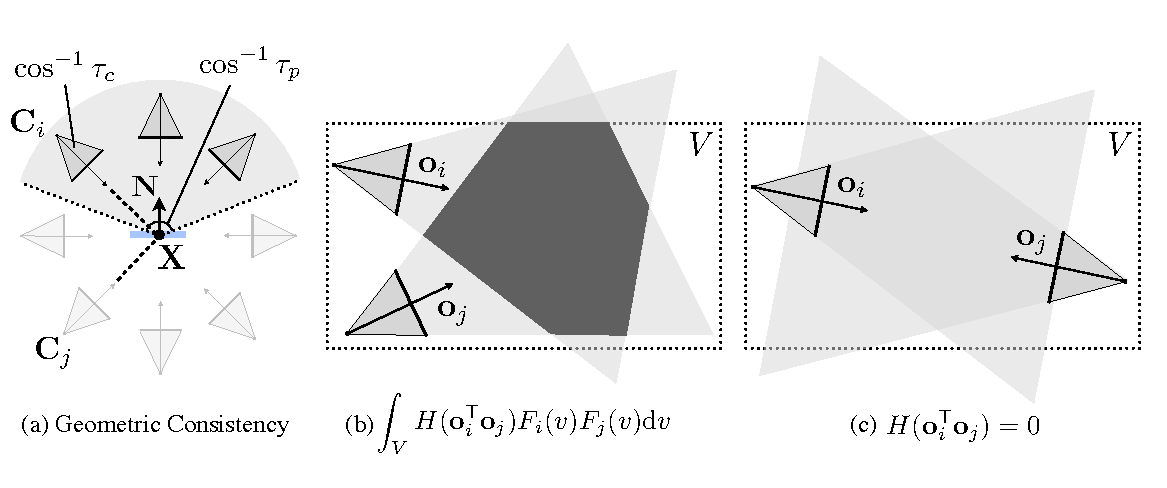
\includegraphics[width=1\columnwidth]{figures/NormalConstraint}
	\caption{(a) The valid region filtered by  $\gamma_p$ and $\tau_p$ is shown as a shaded region. The angle limitation with respect to the $\mathbf{N}$ is computed as $\cos^{-1}{\tau_p}$. (b) 
		$g_\textrm{s}$ computed by two cameras are shown as a shaded polygon, where $\int_V \mathcal{H} (\mathbf{o}_i^{\mathsf{T}} \mathbf{o}_j) F_i(v) F_j(v) {\textrm d}v >0$. (c) An example where $\mathcal{H} (\mathbf{o}_i^{\mathsf{T}} \mathbf{o}_j)=0$ is shown. An oriented patch cannot be visible by two cameras facing each other simultaneously.}
	\label{fig:PatchRelationMRF}
\end{figure}



\subsection{Geometric consistency} \label{sub:Normal-cue}

Oriented patches are only visible from cameras whose ``look-at" vector $\mathbf{o}_i$ is in the opposite direction to the patch normal $\mathbf{N}$ and in front of it. We incorporate this geometric cue based on the co-visibility set $\mathbf{\Gamma}_i$ considering the camera position relative to the patch normal direction and the patch position relative to the camera ``look-at" vector. The probability of $\mathbf{\Gamma}_i$, given visibility $\mathbf{v}_i$, can be written as 
%(We will show a couple of exceptional cased in our experimental results), i.e., camera view angle with respect to the current patch normal:
\begin{eqnarray}
P(\mathbf{\Gamma}_i | \mathbf{v}_i ) = \begin{cases} \frac{1}{ (1- \tau_c)(1- \tau_p)} & {\textrm if~} \gamma_i^c \geq \tau_c,{\textrm and~} \gamma_i^p \geq  \tau_p  \\
0 & {\textrm otherwise,}\end{cases} 
%P(\mathbf{C}_i ~|~ \mathbf{v}_i = 1) &=& \begin{cases} \frac{1}{\rho} & {\rm if~} \mathbf{N}^\mathsf{T} \overline{\mathbf{X} \mathbf{C}_i}  > \tau\\\
%                                                           0 & {\rm otherwise.}\end{cases}
%P(\mathbf{c}_i ~|~ \mathbf{v}_i = 1) &=& T(o_t^{\mathsf{T}}n_i < \theta) / \tau
\label{eq:eq_normal}
\end{eqnarray}
where $\tau_c<1 $ is the cosine angle representing the field of view of the camera, and $\tau_p<1$ is a threshold (cosine angle) to determine the angular visibility with respect to the patch normal. Figure~\ref{fig:PatchRelationMRF}(a) shows an example of the cue, where the shaded area represents the valid region according to $\tau_p$.

%where $\overline{\mathbf{X} \mathbf{C}_i}$ is a unit vector from target point (patch center) to the camera center, $\rho$ is a normalization factor so that sum of the distribution becomes one. $\tau$ is threshold to determine a angle limitation where the patch is visible. 

\subsection{Visibility Regularization Prior} \label{sub:prior}
Under a Markov Random Field prior over camera visibility, we decompose the joint probability of visibility $P(\mathbf{V})$ into pairwise probabilities, i.e.,
\begin{eqnarray}
P(\mathbf{v}_1, \cdots, \mathbf{v}_N)= \prod_{i,j \in \mathcal{G}(i)} P(\mathbf{v}_i, \mathbf{v}_j),
\end{eqnarray}
where $\mathcal{G}(i)$ is the set of adjacent camera indices of the $i^{\textrm th}$ camera. This decomposition captures the prior distribution of visibility, representing the prior that two cameras that have similar viewpoints are likely to have consistent visibility. This proximity constraint constitutes prior knowledge that can regularize noisy visibility when both photometric consistency and motion consistency cues are weak (e.g., due to motion blur in an individual camera). We model the log likelihood of the joint probability as follows:
\begin{eqnarray}
\log P(\mathbf{v}_1, \cdots, \mathbf{v}_N) \propto \sum_{i,j \in \mathcal{G}(i)} g_s (\mathbf{v}_i,\mathbf{v}_j),
\label{eq:eq_mrf}
\end{eqnarray}
where $g_s$ is defined by the cost between two cameras using the overlapping volume of the two camera frustums. This is estimated as follows:
\begin{eqnarray}
g_\textrm{s}(\mathbf{P}_i,\mathbf{P}_j) = \frac{\int_V \mathcal{H} (\mathbf{o}_i^{\mathsf{T}} \mathbf{o}_j) F_i(v) F_j(v) {\textrm d}v} {\int_V F_i(v) + F_j(v) - F_i(v)F_j(v) {\textrm d}v}, 
%g_\textrm{s}(\mathbf{P}_i,\mathbf{P}_j) = \frac{|\int_V \mathcal{H} (\mathbf{o}_i^{\mathsf{T}} \mathbf{o}_j) F_i(v) F_j(v) {\rm d}v|^2}{\int_V F_i(v) {\rm d}v \int_V F_j(v) {\rm d}v},
\end{eqnarray}
where $v$ is an infinitesimal volume in the working space $V$ (see Figure~\ref{fig:PatchRelationMRF}(c)). $F_i(v)$ is a binary function defined as 
\begin{eqnarray}
F_i(v) = \begin{cases} 1 & {\textrm if~}v~{\textrm is~visible~from~the~}i^{\textrm th} {\textrm~camera}
\\ 0 & {\textrm otherwise.}
\end{cases}
\end{eqnarray}
$\mathcal{H}$ is a Heaviside step function to take into account a pair of cameras oriented in similar directions. Equation~(\ref{eq:eq_mrf}) captures the ratio between the volume of the intersections of camera frustums and the volume of the union of camera frustums. Figure~\ref{fig:PatchRelationMRF}(b) illustrates $g_\textrm{s}$ where the shaded polygon represents $\int_V \mathcal{H} (\mathbf{o}_i^{\mathsf{T}} \mathbf{o}_j) F_i(v) F_j(v) {\textrm d}v$, and Figure~\ref{fig:PatchRelationMRF}(c) shows an example where $\mathcal{H} (\mathbf{o}_i^{\mathsf{T}} \mathbf{o}_j)=0$.

%i.e.,
%\begin{eqnarray}
%\mathccal{H}(o_i,o_j) = \begin{cases} 1 & {\rm if~} o_i^\matthsf{T}o_j >0
%					\\ 0 & {\rm otherwise.}
%		\end{cases}
%\end{eqnarray}

In practice, we discretize the working volume using voxels and count the number of common voxels that are projected inside both cameras. This enables us to reward consistent visibilities in proximal cameras. %Figure~\ref{fig:MRF}(b) and (c) shows examples of camera relation and computed edge cost. %, and Figure~\ref{fig:MRF}(b),(c) show the generated camera graph in our system setup with calculated edge cost. 

\subsection{MAP Visibility Estimation via Graph Cuts\label{sub:graphcuts}} 
We incorporate Equations~(\ref{eq:eq_appearance}), (\ref{eq:eq_motion}), (\ref{eq:eq_normal}), and (\ref{eq:eq_mrf}) into Equation~(\ref{eq:goalFunction}) to find the MAP estimate of visibility $\mathbf{V^*}$ and, therefore, Equation~(\ref{eq:goalFunction}) can be rewritten as:
\begin{eqnarray}
\mathbf{V^*} = \underset{\mathbf{V}}{\operatorname{argmin}}  \sum_{i=1}^{N} E_d( \mathbf{v}_i) + \sum_{ i, j \in \mathcal{G}(i) } E_s (\mathbf{v}_i,\mathbf{v}_j),
\end{eqnarray}
where $E_d$ encodes photometric consistency, motion consistency, and geometric consistency, and $E_s$ encodes the prior between cameras. 
%\begin{eqnarray}
%E_d(\mathbf{v}_i) =& \frac{\| \mathbf{m}_i - ( \mathbf{x}_i(t) - \mathbf{x}_i(t-1) )  \|^2} {2\sigma^2} -\kappa {\mathbf{Q}_i}^\mathsf{T} \mathbf{q}_i + \delta(\gamma_i ) \nonumber\\
%E_s(\mathbf{v}_i,\mathbf{v}_j) =& \begin{cases} -g_\textrm{s}(\mathbf{P}_i,\mathbf{P}_j) & {\rm if~} \mathbf{v}_i=\mathbf{v}_j  \nonumber\\                                                             
%0 & {\rm otherwise,}\end{cases} 
%\end{eqnarray}
\begin{eqnarray}
E_d(\mathbf{v}_i) =& \frac{\| \mathbf{m}_i - ( \mathbf{x}_i(t) - \mathbf{x}_i(t-1) )  \|^2} {2\sigma^2} -\kappa {\mathbf{Q}_i}^\mathsf{T} \mathbf{q}_i + \delta(\mathbf{\Gamma}_i ) \nonumber\\
E_s(\mathbf{v}_i,\mathbf{v}_j) =& \begin{cases} 0 & {\textrm if~} \mathbf{v}_i=\mathbf{v}_j  \nonumber\\                                                             
g_\textrm{s}(\mathbf{P}_i,\mathbf{P}_j) & {\textrm otherwise,}\end{cases} 
\end{eqnarray}
where $\delta = \log(1-\tau_c)(1-\tau_p)$  if $\gamma_i^c > \tau_c$ and $\gamma_i^p>\tau_p$, or $\delta=\infty$, otherwise. This minimization problem can be optimally computed via graph cuts~\cite{boykov2001fast}. 
%originates from the distribution related to patch's normal direction (Equation~\ref{eq:distributionNormal}). $\delta$ is infinity value when $P(\mathbf{C}_i ~|~ \mathbf{v}_i = 1) = 0$, or zero otherwise. 

\begin{figure}[t]
	\centering       
	%  \subfigure[An input image]{\label{Fig:visEx_target}\includegraphics[height=0.15\textwidth]{Target}}
	\subfloat[Selected patch]{\label{Fig:visEx_Input}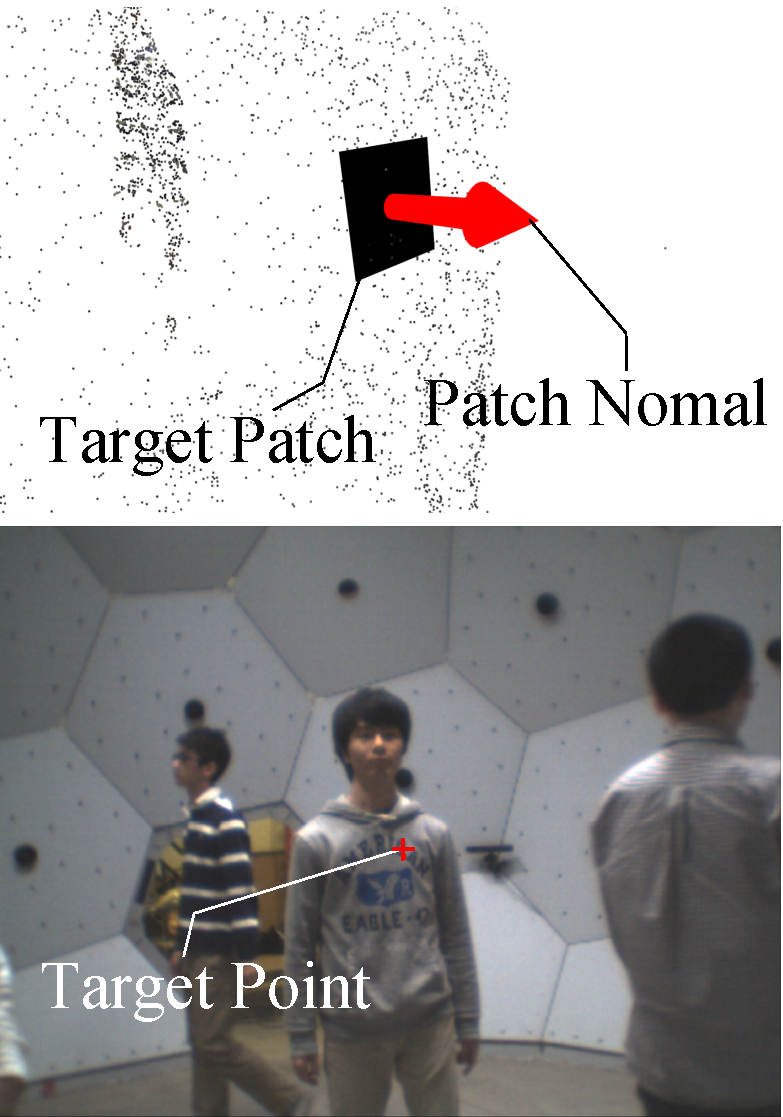
\includegraphics[height=0.2\textwidth]{figures/GT_input_final}}
	\subfloat[Ground truth]{\label{Fig:visEx_GT}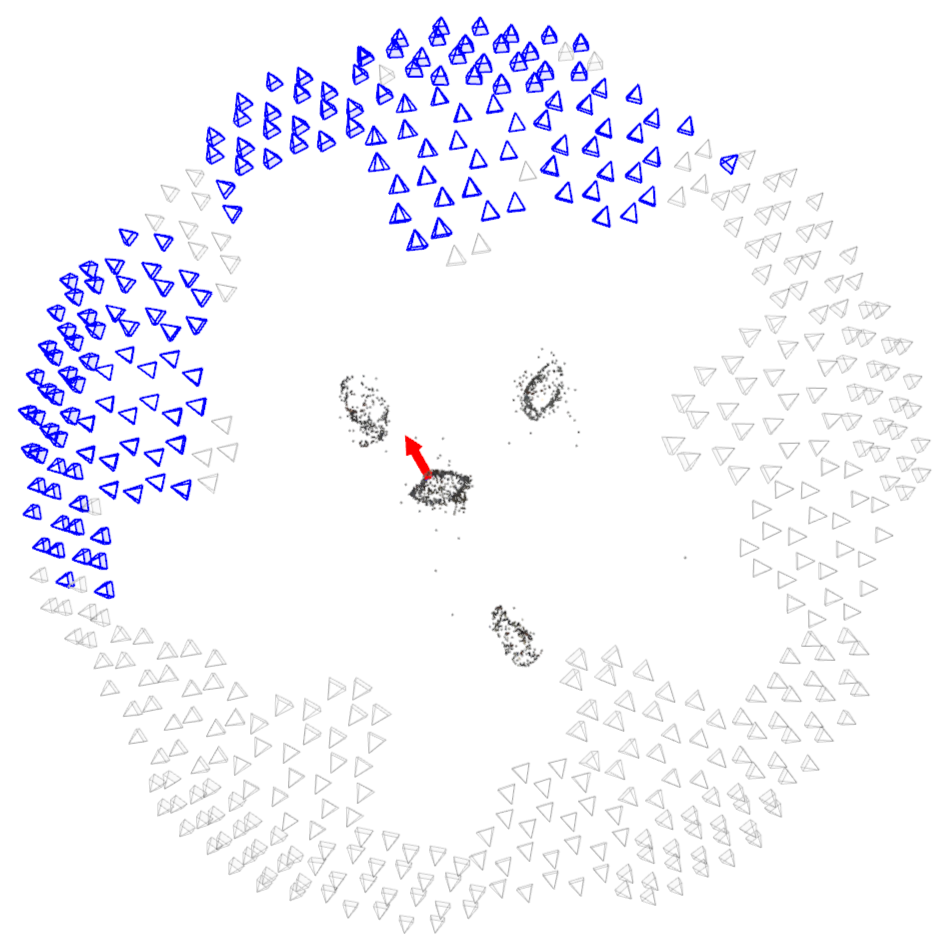
\includegraphics[height=0.2\textwidth]{figures/GT}}
	\subfloat[Photo-consistency]{\label{Fig:visEx_App}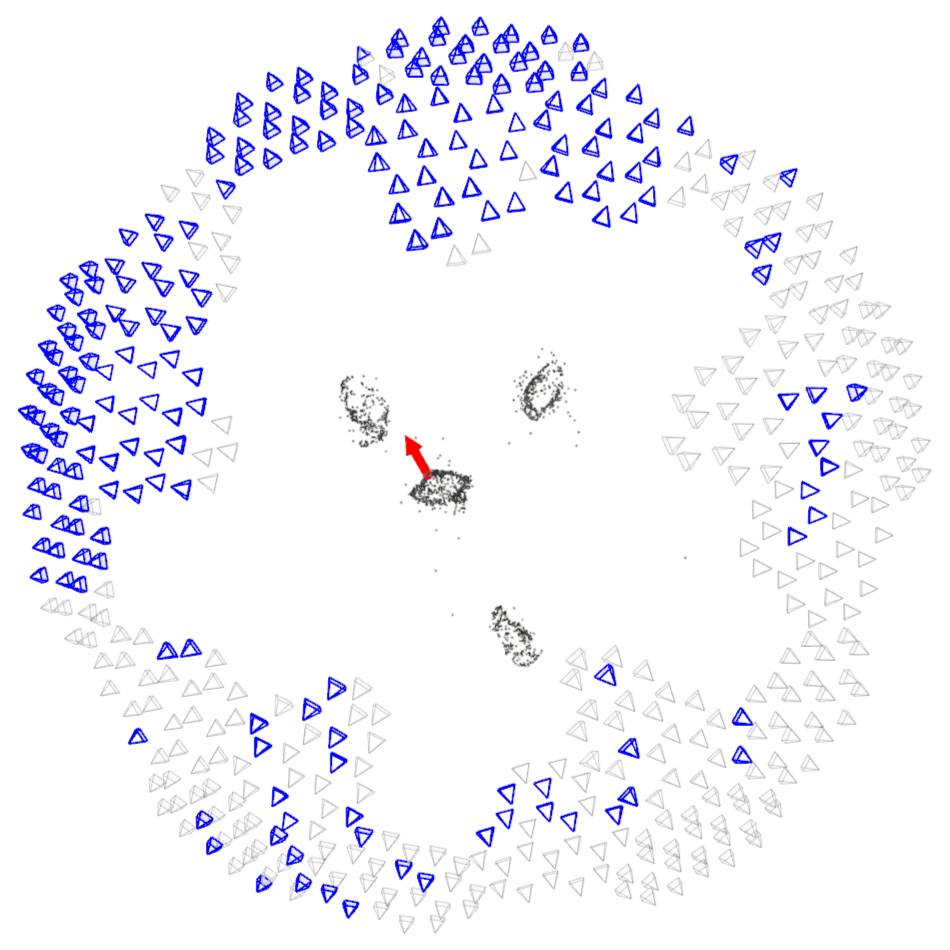
\includegraphics[height=0.2\textwidth]{figures/AppOnly}} 
	\subfloat[MAP] {\label{Fig:visEx_MAP}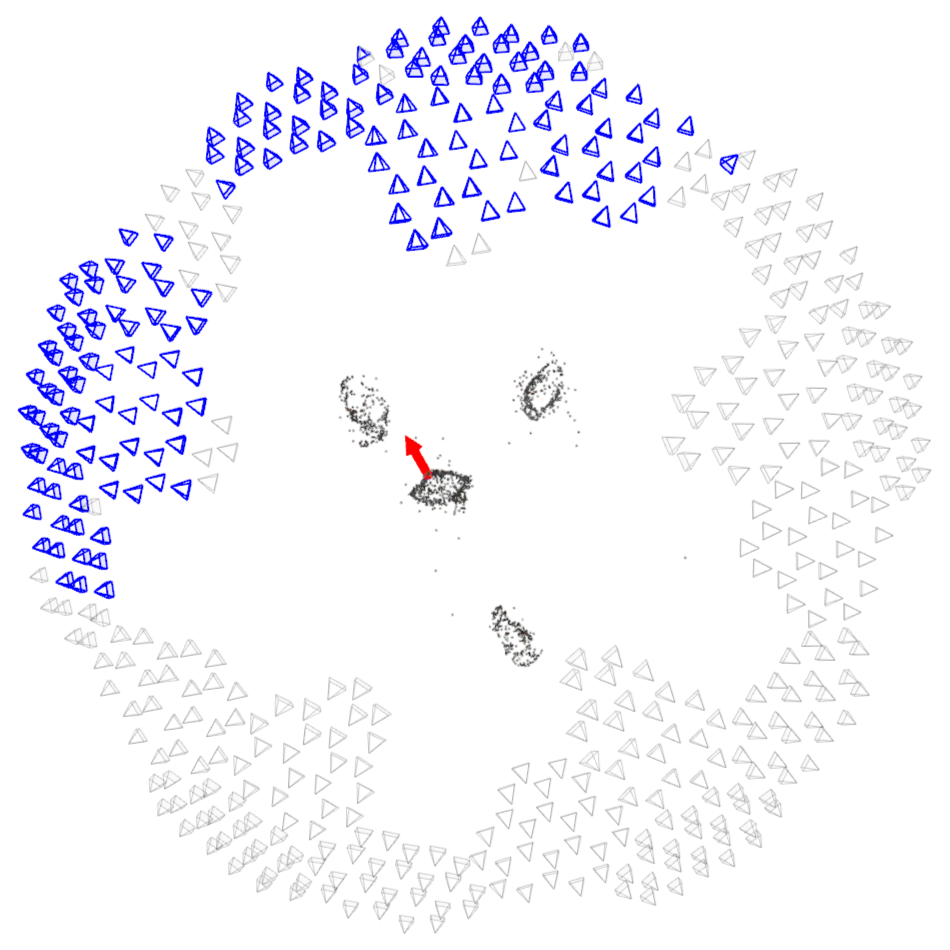
\includegraphics[height=0.2\textwidth]{figures/MAP}} 
	\subfloat[Visibility Accuracy Comparison]{\label{Fig:VisibilityError}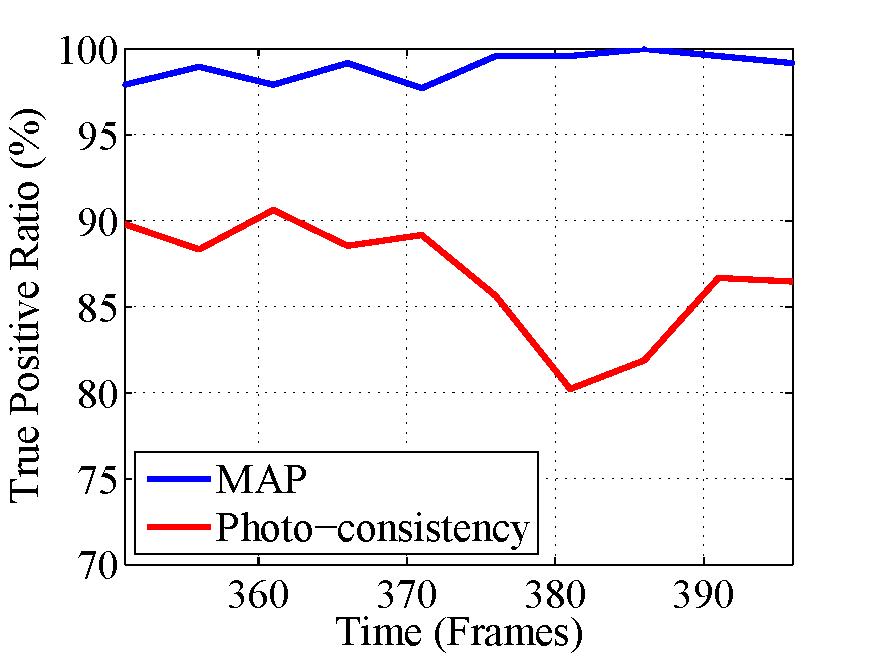
\includegraphics[height=0.2\textwidth]{figures/VisibilityError2}}
	%    \subfigure[Failure case of MAP estimate]{\label{Fig:MAP_failure}\includegraphics[height=0.22\textwidth]{MAP_failure_example}} 
	\caption{The red arrow denotes the normal vector of the selected patch. The pyramid structures represent camera poses, where blue cameras belong to the visible set (we warp the camera positions for better visualization). (a) The selected patch is shown in 3D and 2D image. (b) We manually generate ground truth visibility. (c) Visibility estimated by the baseline. (d) Visibility estimated by our method. (e) We compare accuracy of visibility estimates of both methods.} 
	\label{Fig:visibilityError}
\end{figure}

\section{Results}
% \begin{figure}
% \includegraphics[width=1\columnwidth]{images/CameraGraph}

% \caption{Calibrated 480 cameras and their graph }


% \label{fig:CameraGraph}
% \end{figure}


% \subsection{System Setup and Datasets}

We evaluate our algorithm on a variety of challenging scenes in the presence of significant occlusion (Circular Movement and Falling Boxes), large displacement (Confetti and Fluid motion), and topological change (Falling boxes and Volleyball). Our visibility estimation enables us to better leverage a large number of cameras in producing accurate and long trajectories. The dataset used in the evaluation is summarized in Table~\ref{Table:dataset} and is available on the project website. The sequences were captured at the CMU Panoptic Studio~\cite{PanopticStudio2014} containing 480 cameras capturing 640$\times$480 video at 25 Hz. The cameras are extrinsically and intrinsically calibrated, and are synchronized via an external clock.


\begin{table} [t]

\centering
\caption{Summary of the datasets.}\label{Table:dataset}
\resizebox{0.8\textwidth}{!}{
	\begin{tabular}{c|c|c|c|c}
		\hline 
	{Sequence} & {Frames} & {Duration} & {\# of points}  & {Av. traj. length}\tabularnewline
		\hline 
		\hline 
	{Circ. Movement} & {250} & {10.0 sec} & {10433} & {404.9 cm}  \tabularnewline
		\hline 
	{Volleyball} & {210} & {8.4 sec} & {8422} & {326.4 cm} \tabularnewline
		\hline 
	{Bat Swing} & {200} & {8.0 sec} & {3849} & {224.1 cm} \tabularnewline
		\hline 
	{Falling Boxes} & {160} & {6.4 sec} & {17934} & {164.7 cm}\tabularnewline
		\hline 
	{Confetti} & {200} & {8.0 sec} & {10345} & {103.0 cm} \tabularnewline
		\hline 
	{Fluid Motion} & {200} & {8.0 sec} & {3153} & \scriptsize{123.1 cm} \tabularnewline
		\hline 
	\end{tabular} 
}
\end{table}

% foot note for \label{Fig:visibilityError}
%\footnotetext{We warp the camera positions for better visualization.}

\subsection{Quantitative Evaluation}
\noindent\textbf{Visibility Estimation Accuracy.} We select an arbitrary patch in the Circular Movement sequence reconstructed at a time instance, and manually generate ground-truth visibility data at each sampled time instance by selecting cameras where the target patch is visible. We compare our visibility estimation method (MAP) against a baseline method based on photometric consistency alone, which is a cue commonly used by previous approaches~\cite{Carceroni2002,Devernay2006,Furukawa2008}. Visibility estimation results generated from each method at a time instance are visualized in Figure~\ref{Fig:visibilityError}. As a criterion, we compute the true positive detection rate between the ground truth data and $\mathbf{V}(t)$ estimated by both methods. The true positive rate from each method is shown in Figure~\ref{Fig:VisibilityError}, demonstrating that our method outperforms the baseline method by a significant margin.\\ %In particular, almost all of error of the proposed method are caused by the cameras located at extreme view angle with respect to the patch where it is hard to determine the ground truth value. 
\noindent \textbf{Tracking Accuracy and Length.}
We evaluate our method considering both tracking accuracy and trajectory length. Inspired by the evaluation criterion proposed by Furukawa and Ponce~\cite{Furukawa2008}, a test sequence is generated by appending it at the end of itself in reverse order, and the tracking algorithm is performed on the generated sequence. The tracked patches must return back to the original position, if tracking is accurate. In this experiment, the 3D error is defined by the 3D distance between initial and the final locations of the target point. We generate five test sequences using the Circular Movement sequence by changing the duration (10 to 50 frames) from a fixed initial frame. For the evaluation, we count the number of successfully reconstructed trajectories that have less than 2 cm drift error. Figure~\ref{Fig:traj_distance_histo} shows a histogram of the number of trajectories using 480 cameras.  Our MAP estimate method outperforms the method based on photometric consistency in terms of both number of trajectories and length of trajectories. We also perform experiments with different number of cameras by uniformly sampling cameras to examine its impact on tracking success rate. Figure~\ref{Fig:survivedPt} shows how our method leverages a large number of cameras. Note that the number of successfully tracked trajectories increases faster than the method based on photometric consistency. 

\begin{figure}[t]
	\centering       
	\subfloat[Tracking Performance]{\label{Fig:traj_distance_histo}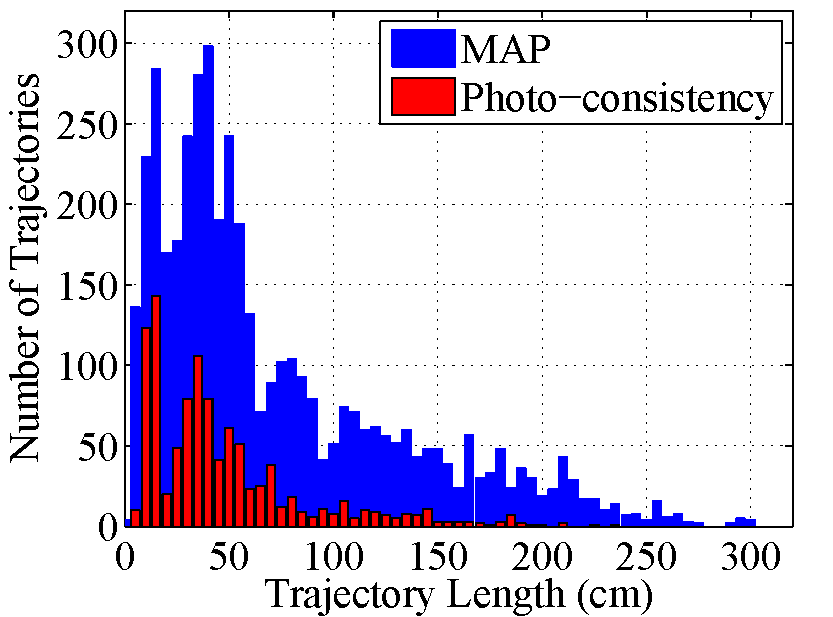
\includegraphics[width=0.4\textwidth]{figures/Circular_Cam480_pt_length3}}
	\subfloat[Number of cameras]{\label{Fig:survivedPt}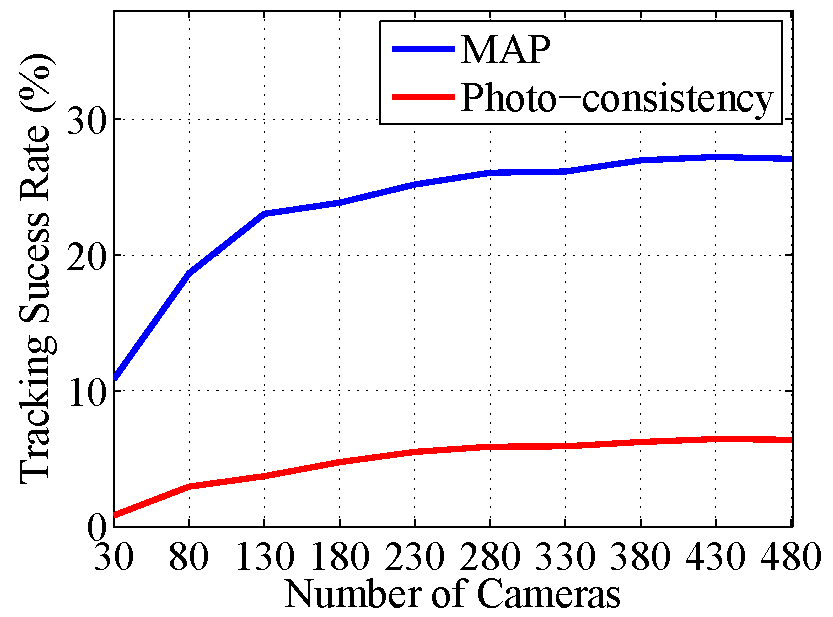
\includegraphics[width=0.4\textwidth]{figures/Circular_PtNum_CamNum3}}     
	\caption{(a) Our MAP estimate outperforms the baseline method in terms of the number of trajectories and the length of trajectories. (b) Our method leverages the large number of views, and shows a faster increasing curve than the baseline method.} 
	\label{Fig:quantitative}
\end{figure}

\begin{figure}[th]
	\centering       
	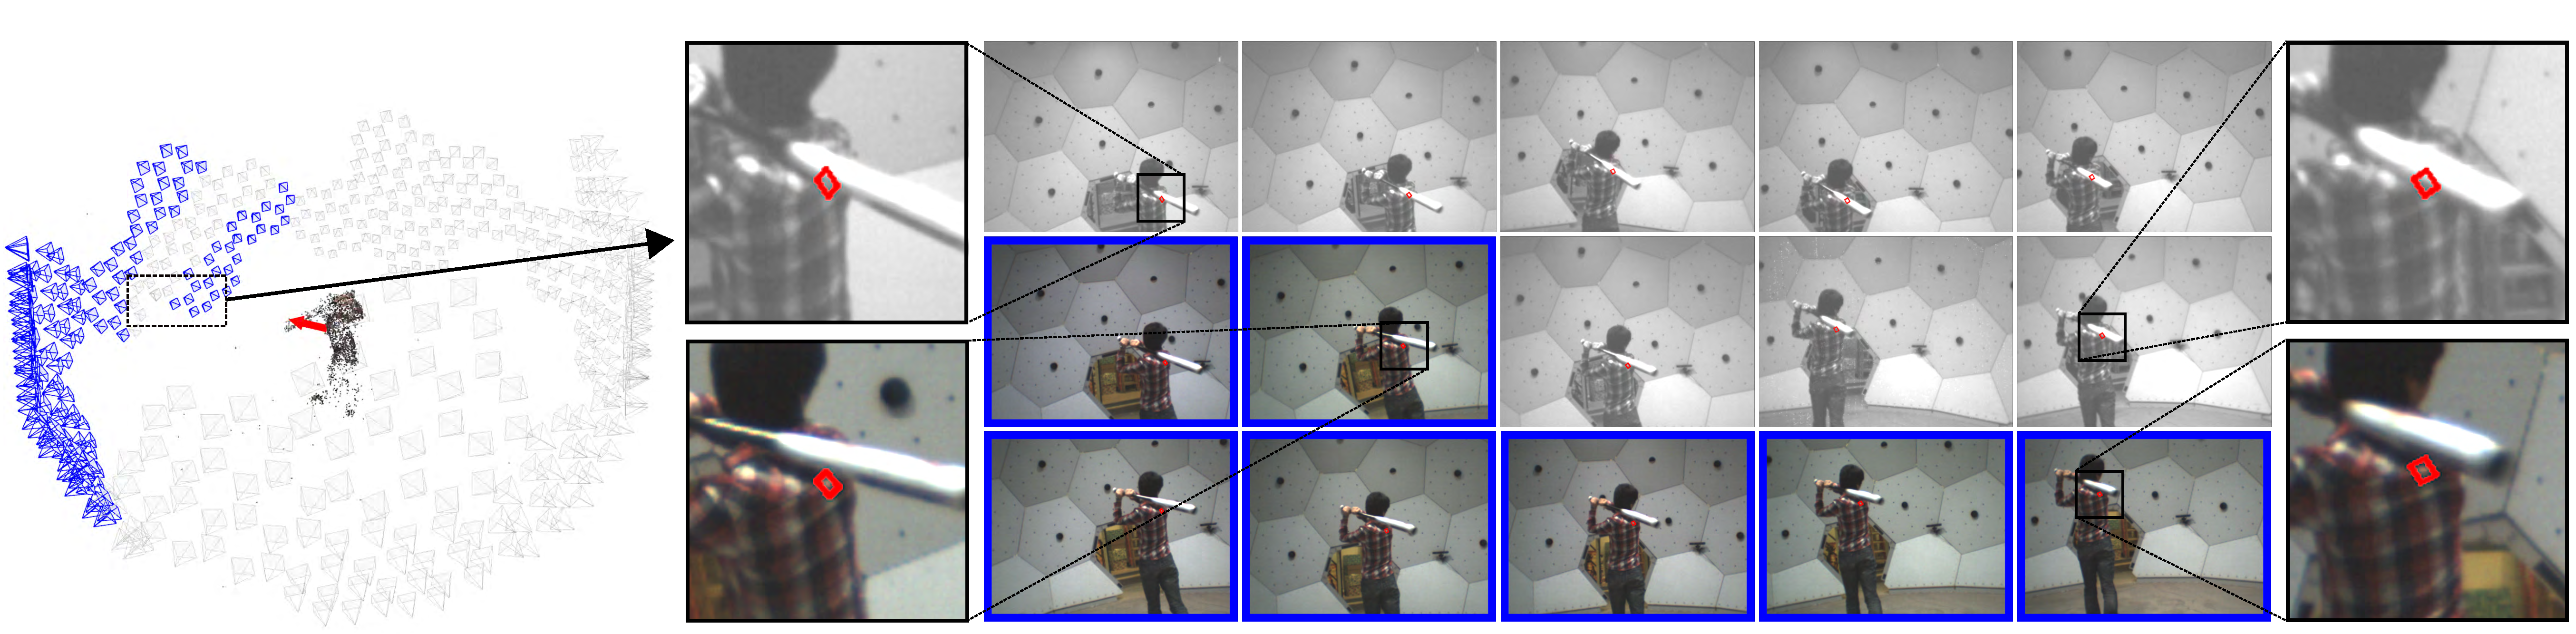
\includegraphics[width=\textwidth]{figures/VisibilityQualitativeFull_small2}
	\caption{We qualitatively demonstrate the performance of MAP visibility estimation using the  sequence. The normal of the selected patch is shown as a red arrow in the 3D view (left) and projected patch is shown as a red polygon in each image (right). The images with a blue boundary are the views that belongs to the visibility set. The bat occludes the patch and its effect can be seen as a ``shadow" on the visibility set of cameras (left).}
	\label{Fig:VisQ}
\end{figure}


\subsection{Qualitative Evaluation}
\noindent \textbf{Visibility Boundary.} We qualitatively demonstrate the performance of our MAP visibility estimation using the  sequence by illustrating cameras in the visibility set in 3D, and showing the projection of the target patch in the images, as shown in Figure~\ref{Fig:VisQ}. This result shows a clean visibility boundary, showing the occluded views by the baseball bat.  

\noindent \textbf{3D Trajectory Recontruction.}
We generate an initial patch cloud for a selected time instance, and perform forwards and backwards patch tracking, up to 150 frames, for all the sequences summarized in Table~\ref{Table:dataset}. Figure~\ref{Fig:qualtitative} shows the reconstructed trajectories. The reconstructed time instances are color coded. Note that our method can be applied multiple times to different time instances to increase the density of the trajectories. \\
\textbf{Circular movement:} Three people rotate around the person at the center (Figure~\ref{Fig:circular}). This experiment is used to evaluate our method in terms of visibility reasoning\\
\textbf{Volleyball:} Two people play volleyball (Figure~\ref{Fig:ball_play}). We demonstrate an event where motion is fast and occlusion is severe. We are able to reconstruct the trajectories of the ball and players.\\
\textbf{:} A person swings a baseball bat. The reconstructed long trajectories can provide a computational basis for sport analytics, capturing subtle motion (Figure~\ref{Fig:baseball}).\\
\textbf{Falling boxes:} A person collides with stacked boxes and the boxes collapse. The scene includes severe occlusion and topological change of the structure (Figure~\ref{Fig:box}).\\
%In this sequence, occlusion is severe because one side of the scene is completely occluded by the stacked boxes. Also the topology of the structure changes significantly where spatial regularity cannot be applied (Figure~\ref{Fig:box}).\\
\textbf{Confetti:} A person throws confetti in the air. 3D reconstruction of such sequences is challenging because of occlusion and appearance changes. Visibility estimation is challenging as the confetti are small and their appearance changes abruptly (Figure~\ref{Fig:confetti}). \\
\textbf{Fluid motion:} We generate turbulent flow in a room using a fan and small confetti (Figure~\ref{Fig:confetti})\footnote{For this result, we turned off geometric consistency by setting $\tau_c = 0$ and $\tau_p = 0$, as the objects are well approximated by planes.}. 
%Our visibility method that leverages a large number of cameras enables us to estimate chaotic motion. This sequence is more challenging than the Confetti sequence because of large displacement, motion blur, and severe interference among the confetti. 
%Our visibility estimation method enables us to reconstruct the chaotic motion of confetti by leveraging the large number of cameras (Figure~\ref{Fig:confetti})\footnote{For this result, we turned off normal cue by setting $\tau = 0$}.


% \begin{comment}
\begin{figure}[t]
	\centering       
	\subfloat[Circular movement]{\label{Fig:circular}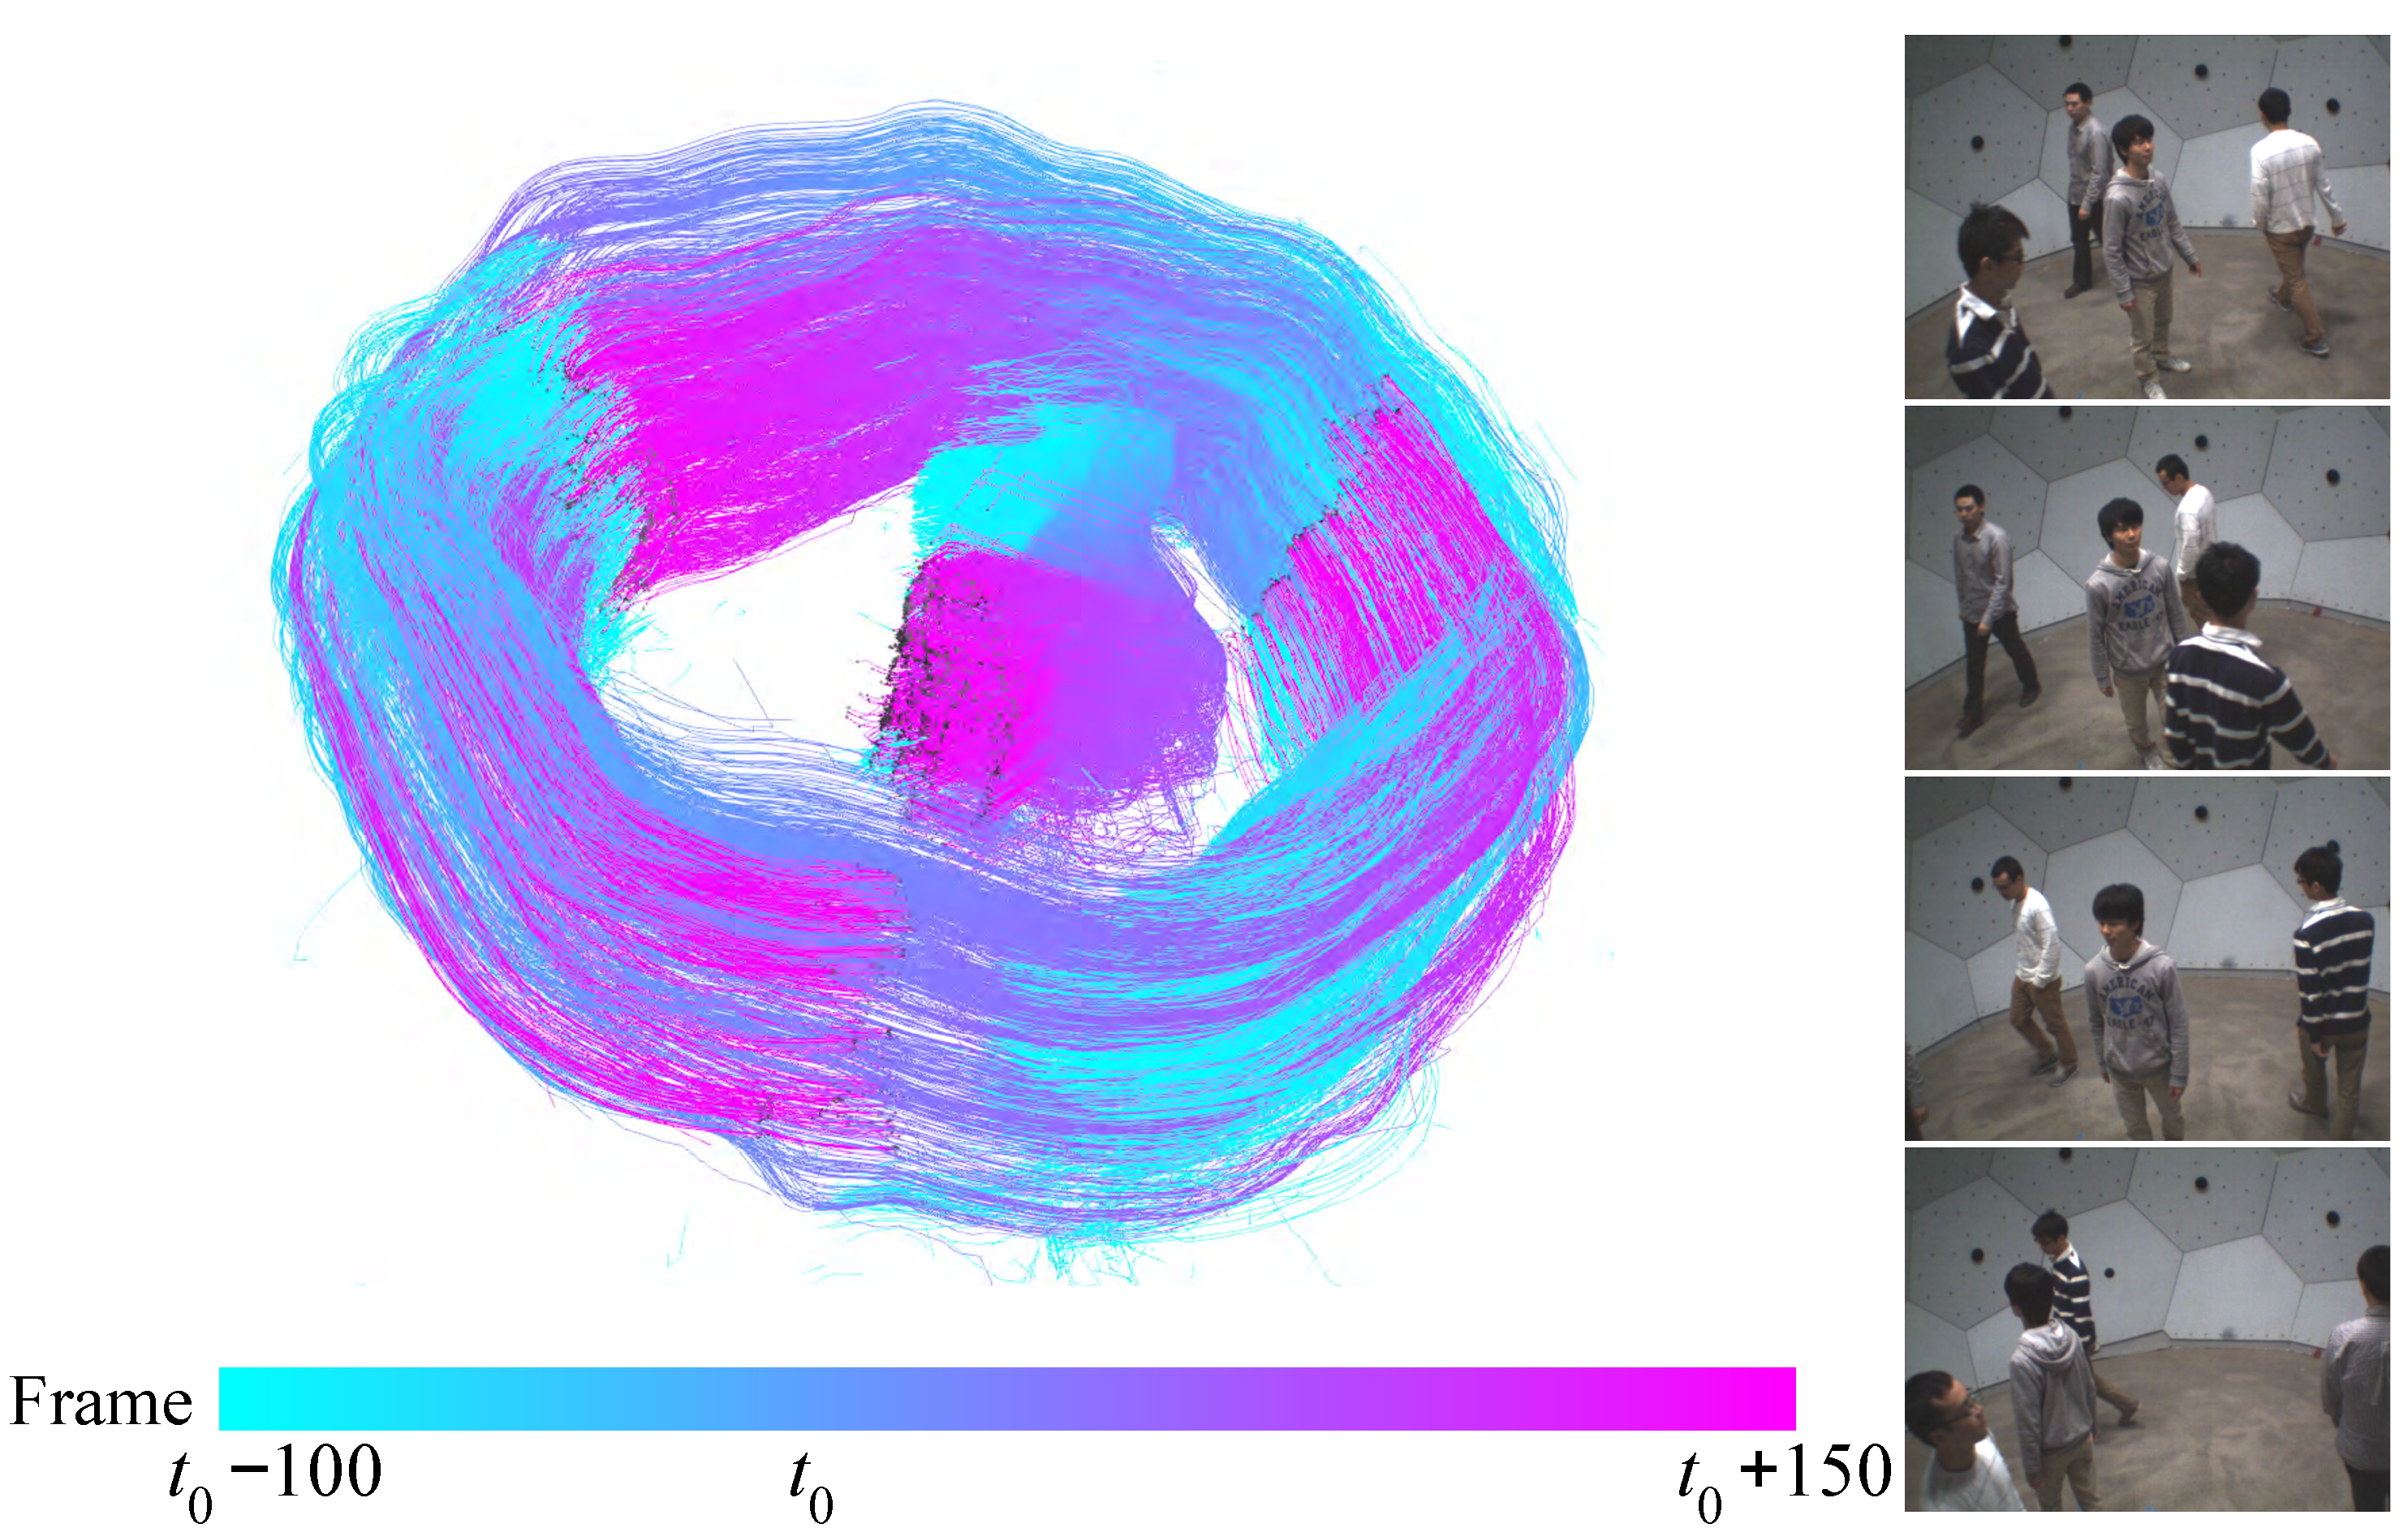
\includegraphics[width=0.45\textwidth]{figures/circle_small}} 
	\subfloat[Volleyball]{\label{Fig:ball_play}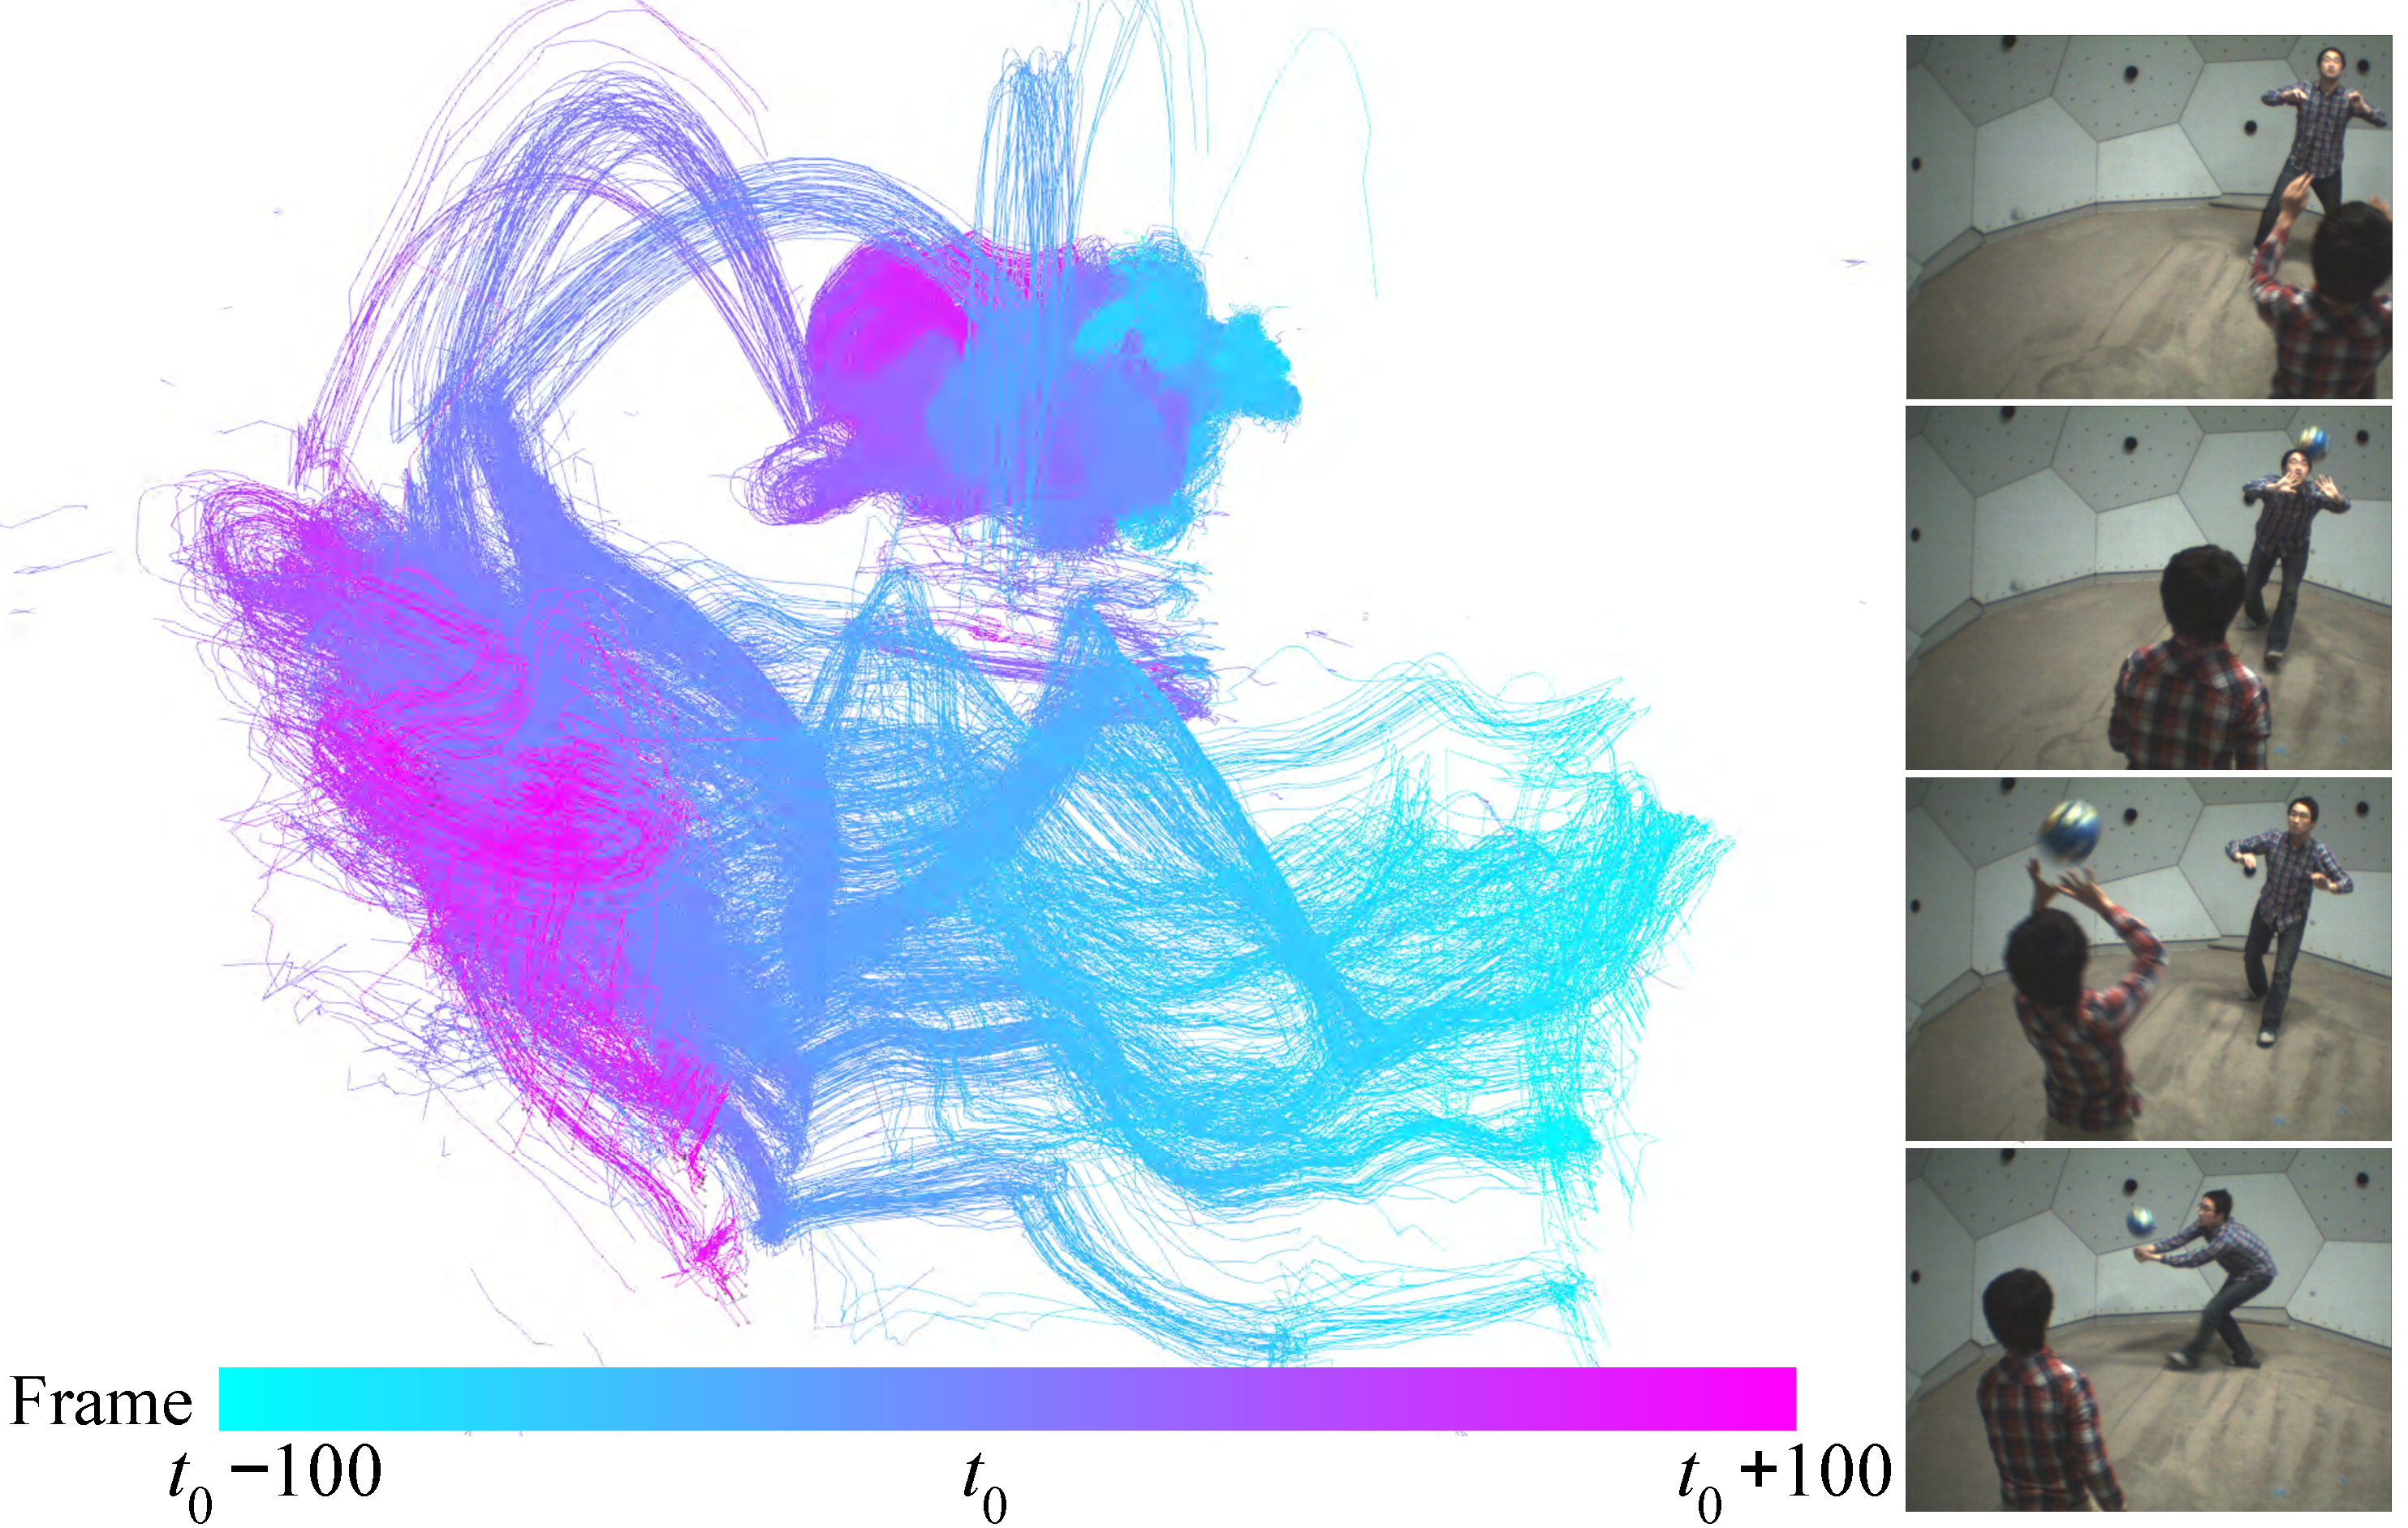
\includegraphics[width=0.45\textwidth]{figures/volleyBall_small}}\\
	\subfloat[Bat Swing]{\label{Fig:baseball}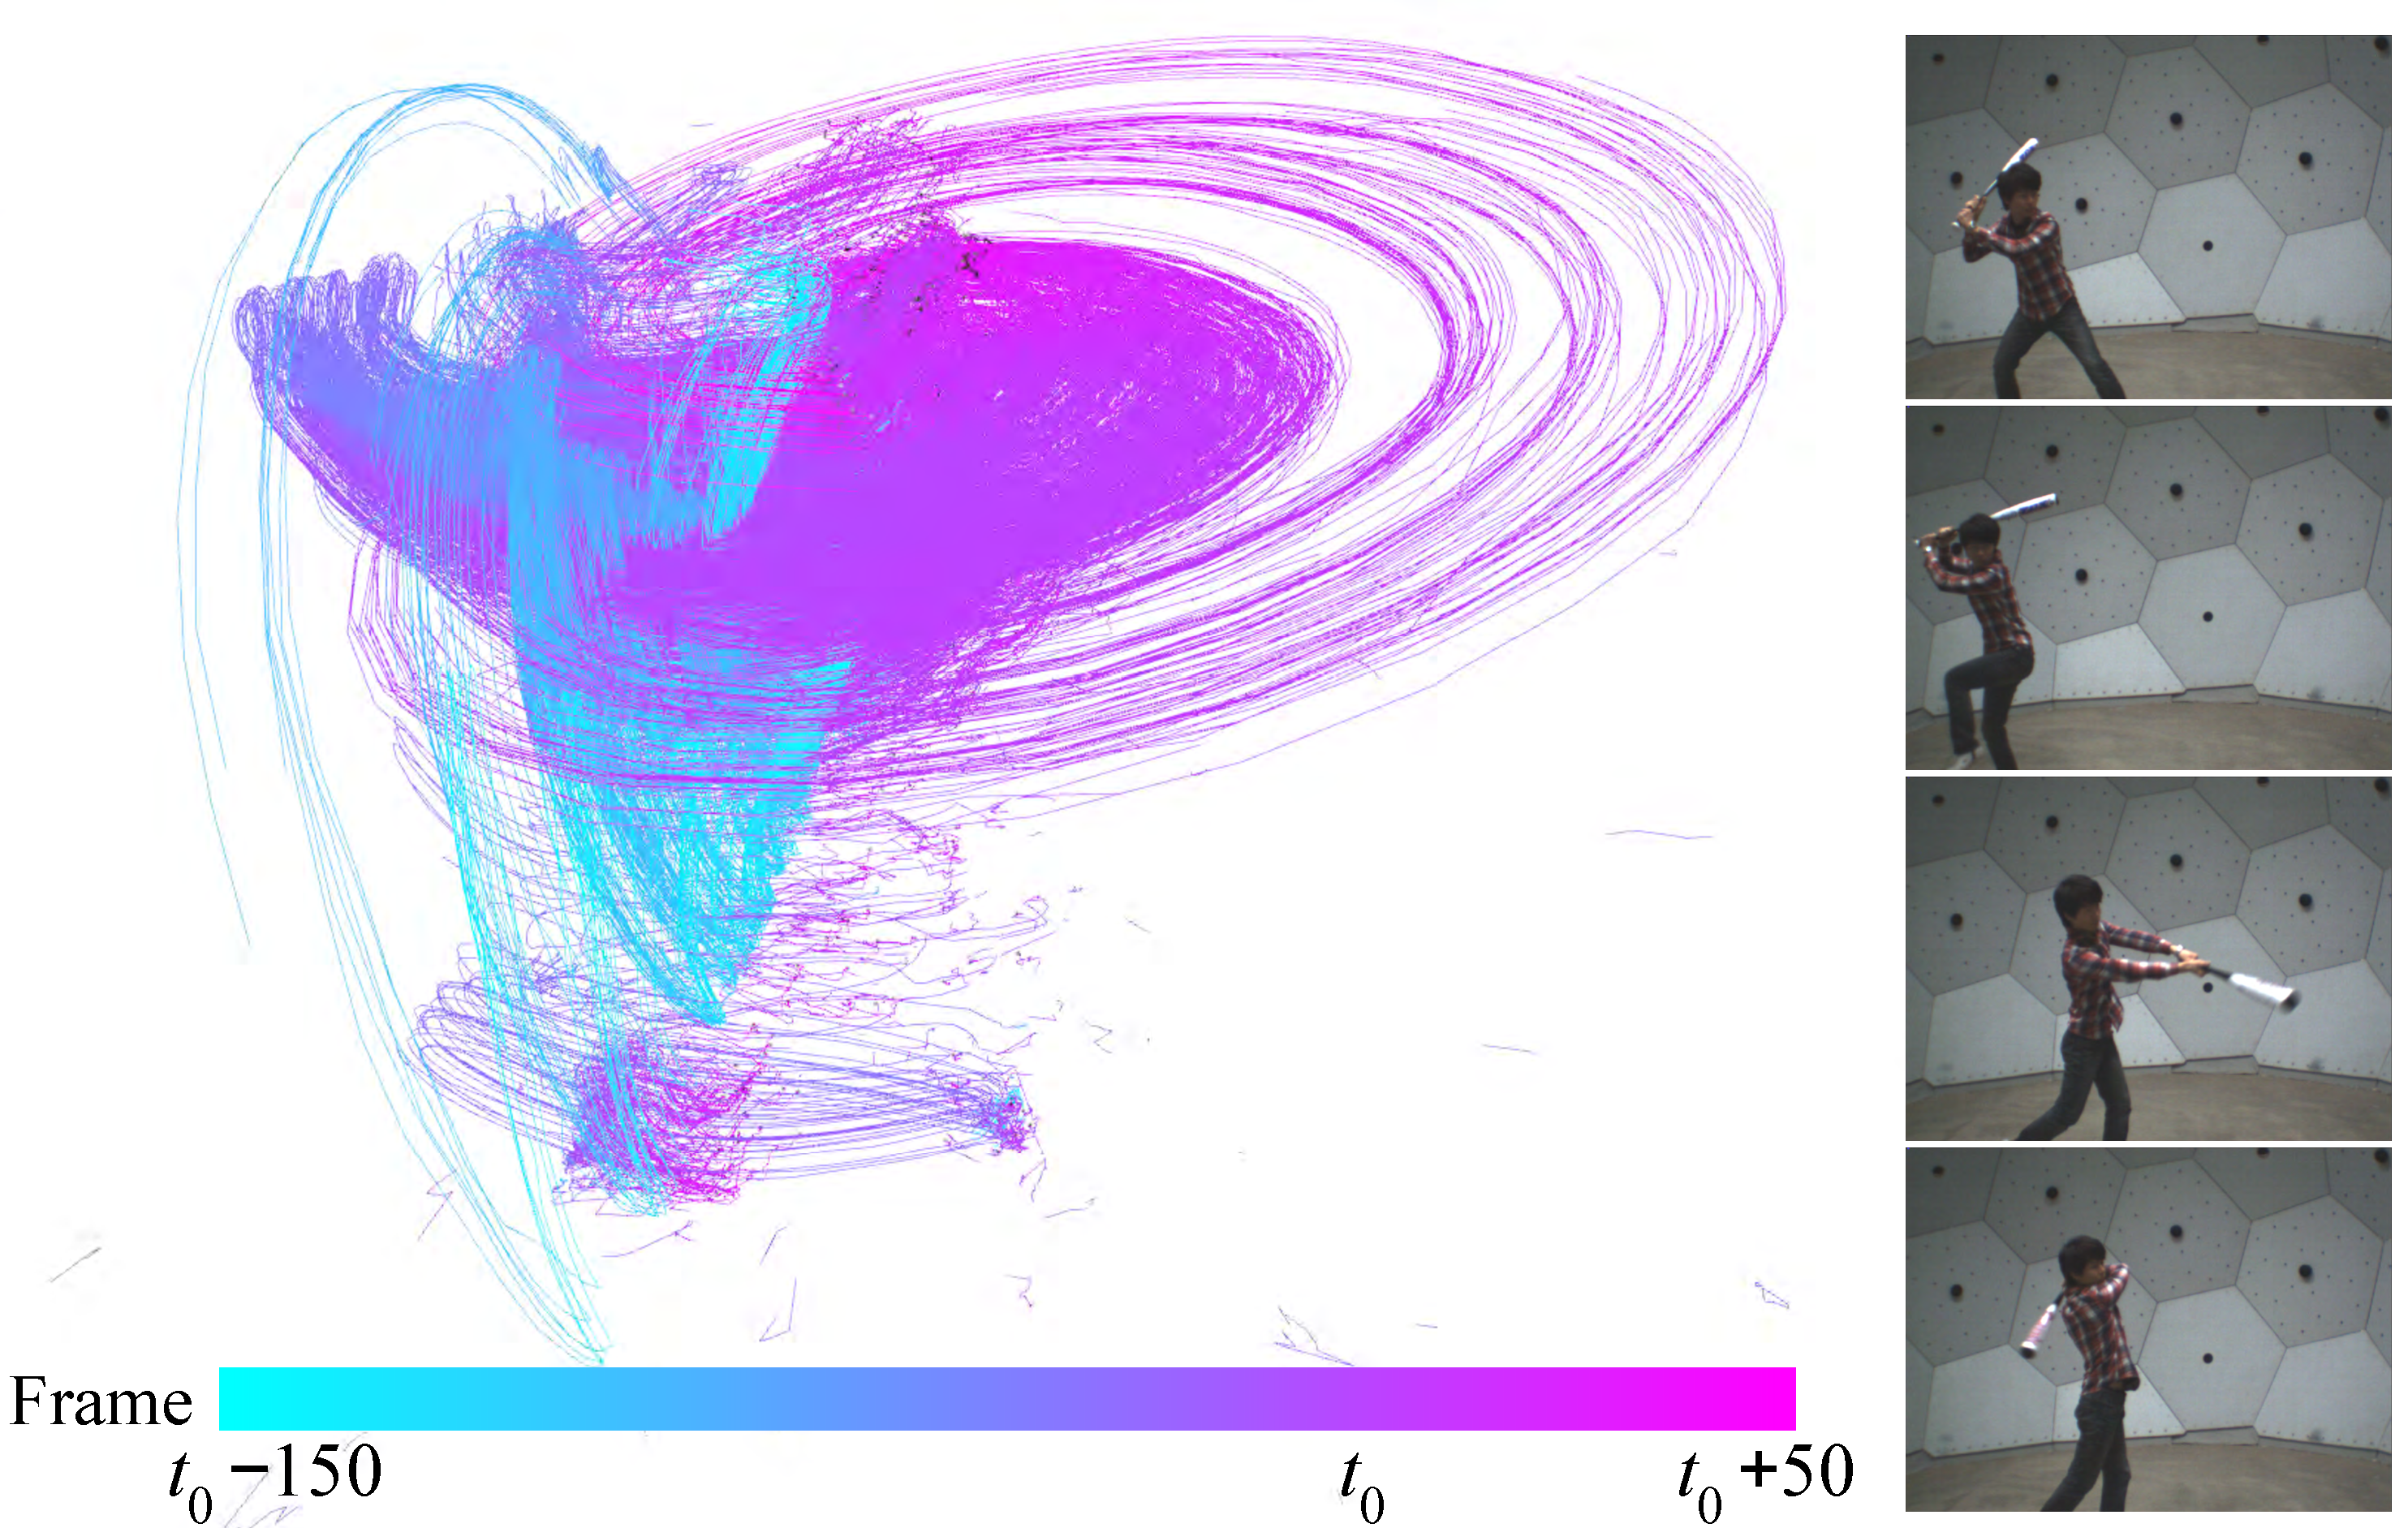
\includegraphics[width=0.45\textwidth]{figures/baseball_small}}
	\subfloat[Falling boxes]{\label{Fig:box}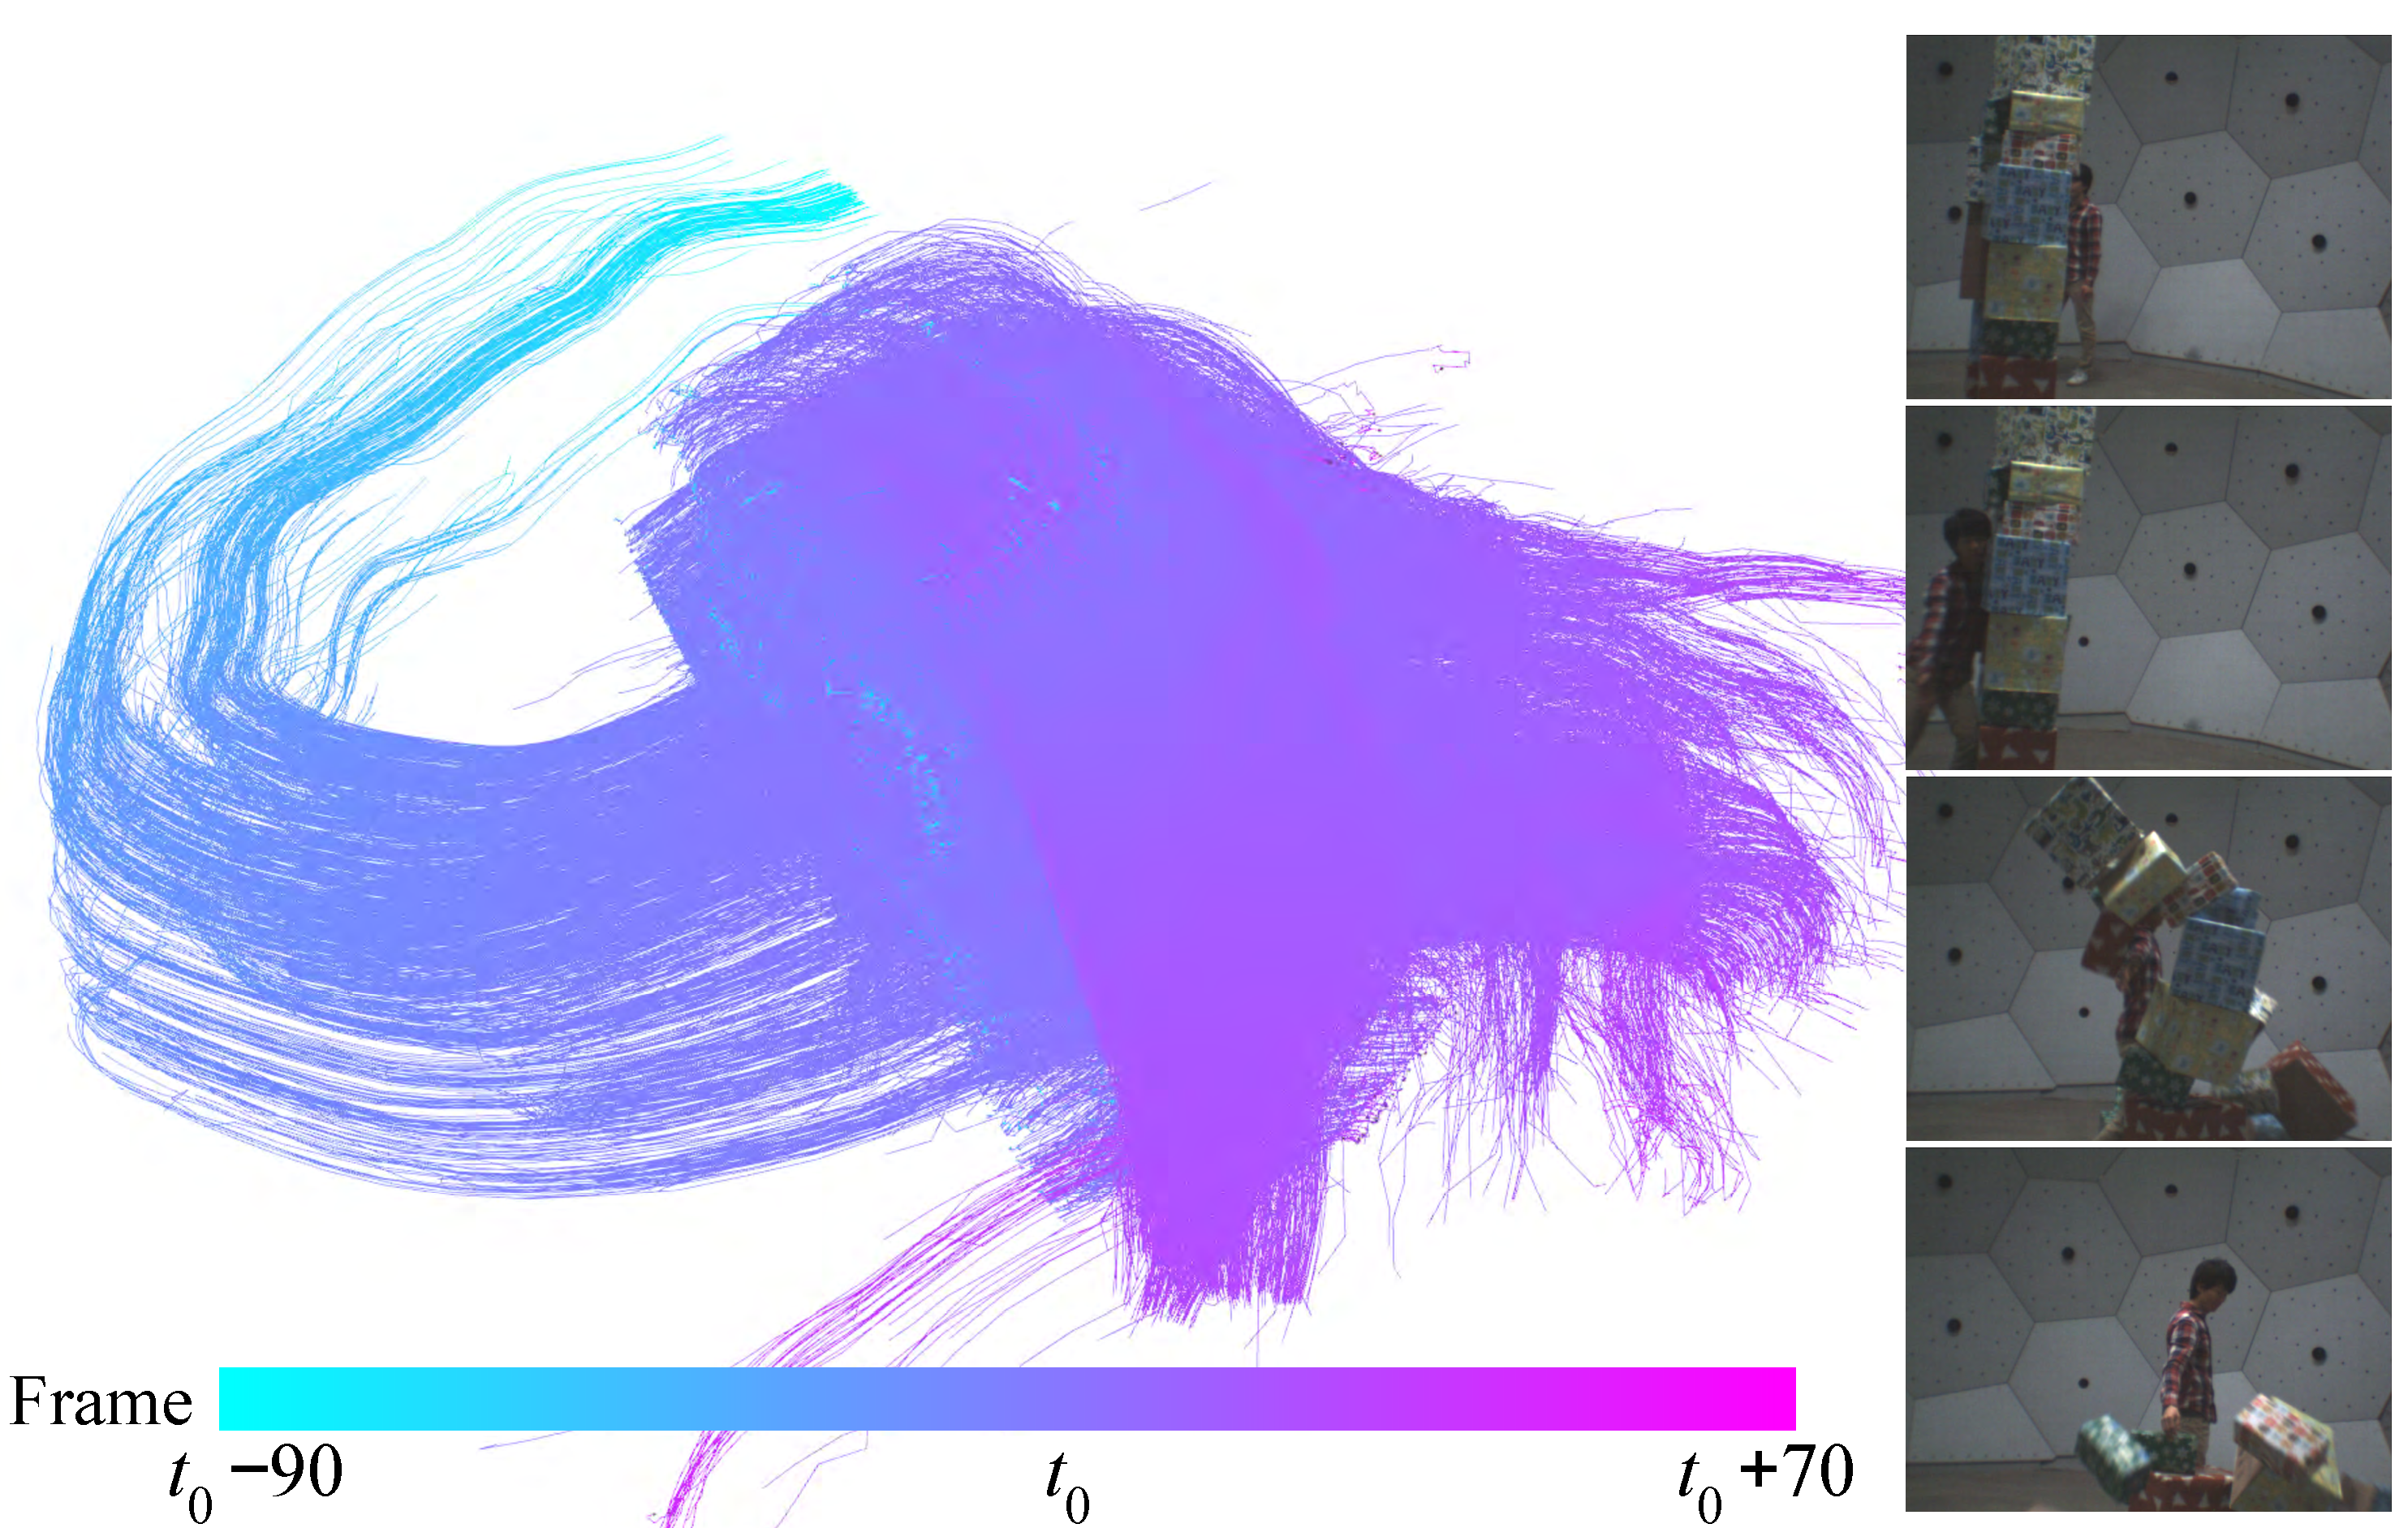
\includegraphics[width=0.45\textwidth]{figures/box_small}}\\
	\subfloat[Confetti]{\label{Fig:confetti}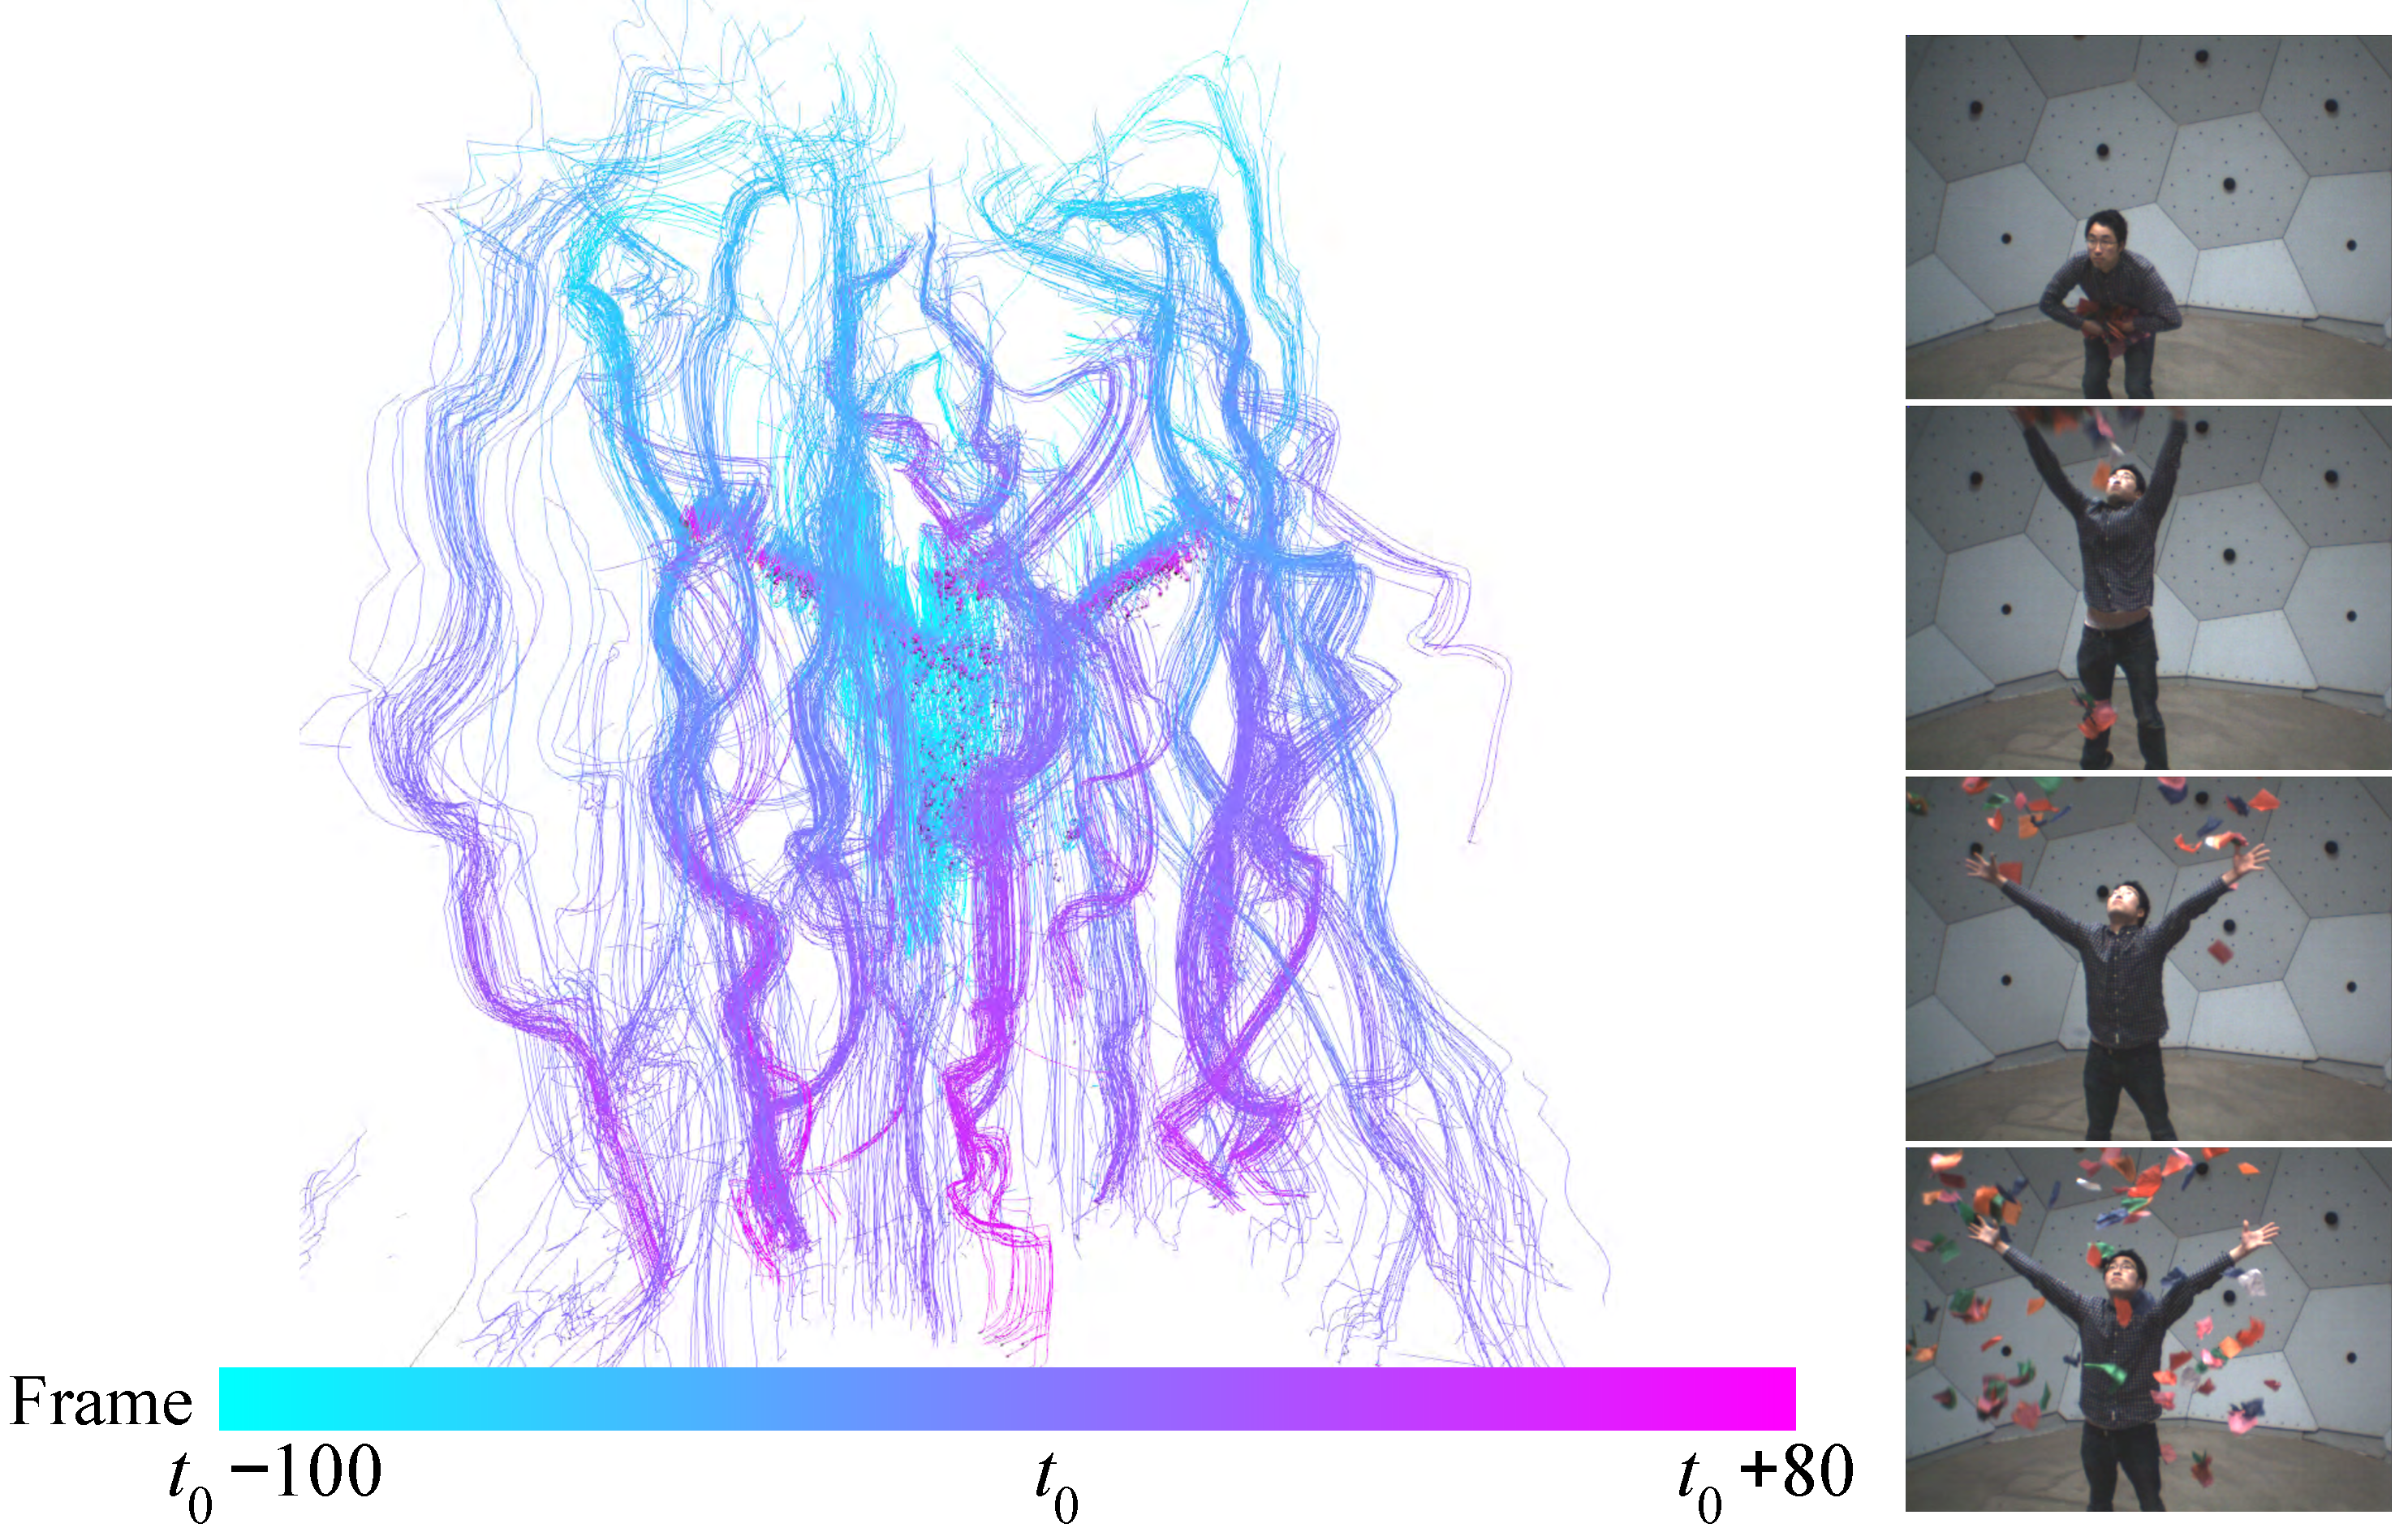
\includegraphics[width=0.45\textwidth]{figures/confetti_small}} 
	\subfloat[Fluid motion]{\label{Fig:fluid_motion}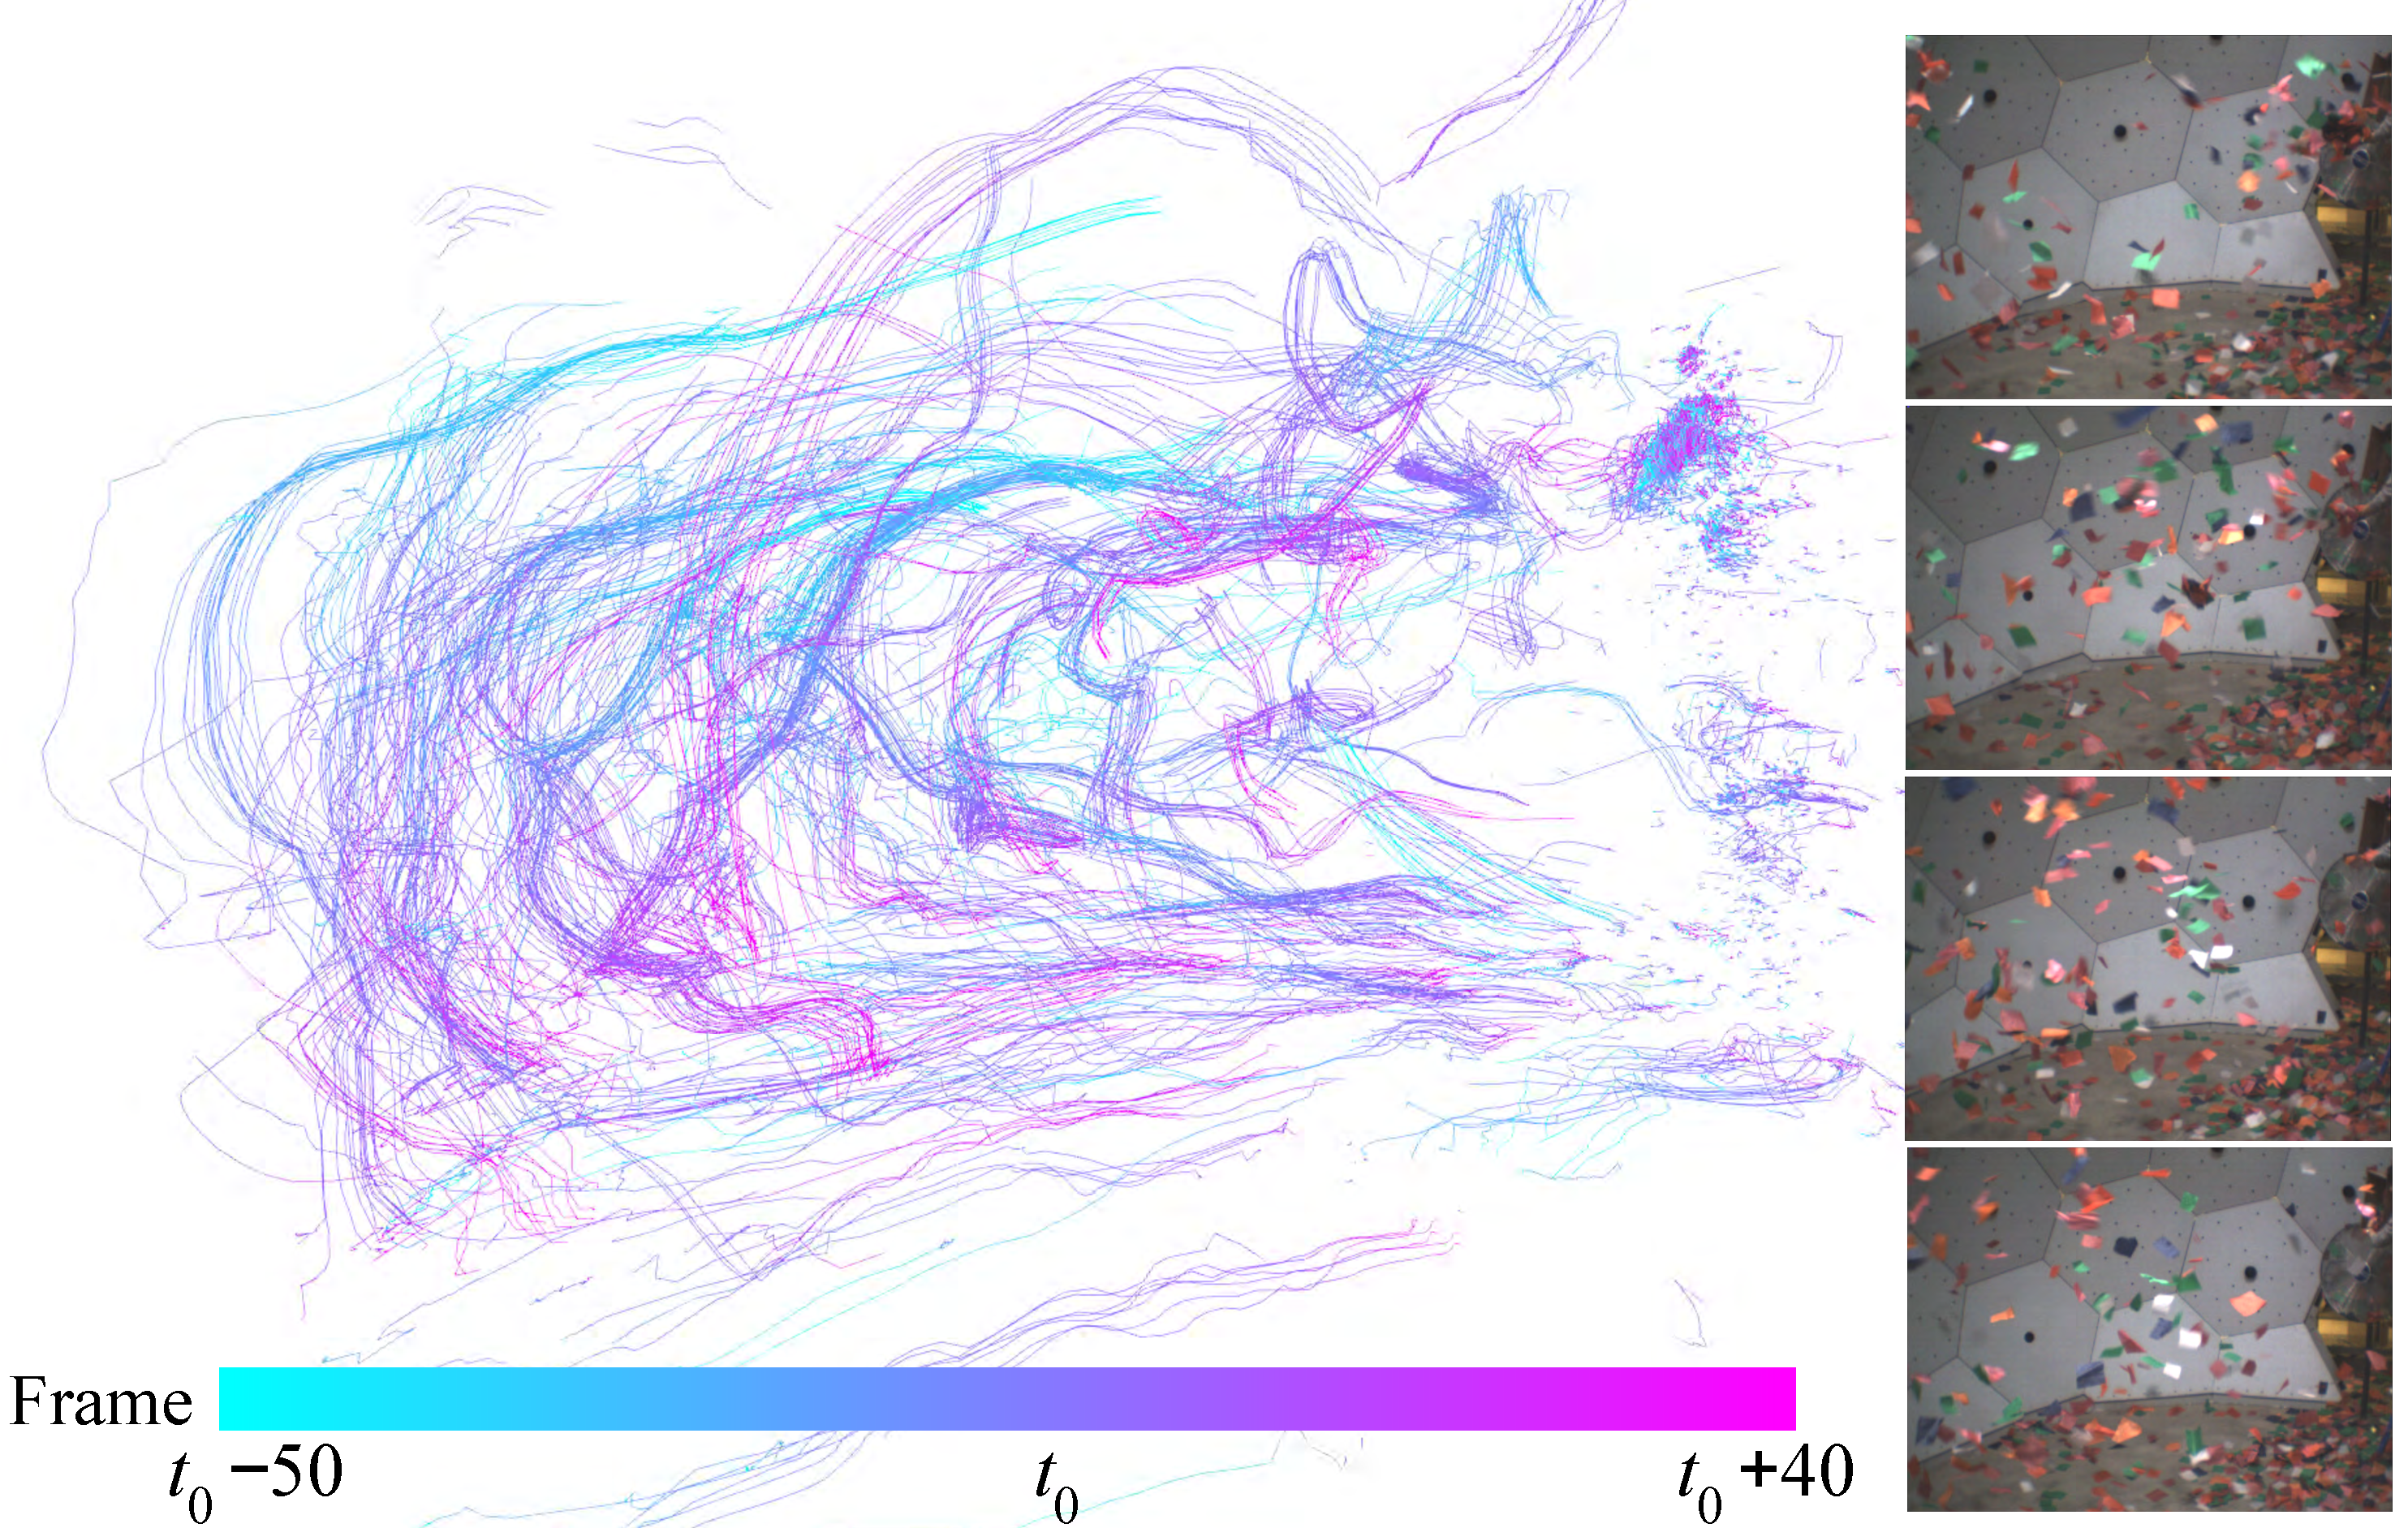
\includegraphics[width=0.45\textwidth]{figures/fluid_small}}   
	\caption{We reconstruct 3D trajectories in real world scenes in the presence of significant occlusion, large displacement, and topological change. The color codes the time that trajectory points are reconstructed. Note that each trajectory is individually reconstructed without any spatial or temporal regularization.} 
	\label{Fig:qualtitative}
\end{figure}
% \end{comment}


\section{Summary}
In this chapter, we present a method to reason about the time-varying visibility for 3D trajectory reconstruction to leverage the large number of views in the Panoptic Studio. We address novel cues (motion consistency, geometric consistency, and visibility regularization prior) for visibility estimation, and fuse them with the commonly used photometric consistency cue, within a MAP estimation framework. We demonstrate that our algorithm provides a more accurate visibility and, consequently, produces longer and denser 3D trajectories than a baseline using only photometric consistency. Unlike the photometric consistency cue, The motion consistency cue is complementary to the photometric cue, as it does not require the texture and the explicit 3D shape of the target 3D patch. Although the motion consistency cue can be ambiguous, this ambiguity, in practice, usually occurs for the cameras behind the target patch when the whole object body (including the patch) undergoes pure translation; this case is handled well by the geometric consistency of the patch and camera. 

A key benefit of our approach is that it does not use any spatial or temporal regularization over the position of the point---the regularization used in our approach is over visibility. This results in ``faithful" reconstruction of 3D point motion that is not biased or smoothed out by prior models of deformation, and this advantage is essential in measuring objective kinesic signals in social situations. 


\pagebreak